\documentclass{jsai2e}

\usepackage[dvipdfmx]{graphicx}
\usepackage{fancybox}
\usepackage{comment}
\usepackage{url}
\usepackage{amsmath}
\usepackage{tabularx}
\usepackage{makecell}

\usepackage{xcolor}

% ===== 表示切り替え =====
\newif\ifshowlabels
\showlabelstrue
% \showlabelsfalse

% ===== 色定義 =====
\definecolor{fixred}{RGB}{200,50,50}
\definecolor{furu}{RGB}{50,50,200}

% ===== 汎用コマンド =====
\newcommand{\tagtext}[3]{%
  \ifshowlabels
    \textcolor{#1}{#3\textsuperscript{\textsf{[#2]}}}%
  \else
    #3%
  \fi
}

% ===== 色＋ラベルのセット =====
\newcommand{\fix}[2]{\tagtext{fixred}{#1}{#2}}
\newcommand{\furu}[2]{\tagtext{furu}{#1}{#2}}
% \showlabelstrue
\showlabelsfalse

%%%%% blindreview廃止に関して（2023/04 Matsubayashi）
%\usepackage{color}
%\def\RED#1{\textcolor{red}{#1}}  

%%%%% LaTeXなどのロゴの定義
\makeatletter
\catcode`\@=11
\font\eightsy=cmsy8
\def\AMSTeX{\leavevmode
\hbox{$\scriptstyle\cal A$}\kern-.25em
 \lower.4ex\hbox{\eightsy M}\kern-.1em{$\cal S$}-\TeX}
\catcode`\@=\active
\def\LaTeX{{\rm L\kern-.36em\raise.3ex\hbox{$\scriptstyle {\rm A}$}\kern-.15em
 T\kern-.1667em\lower.7ex\hbox{E}\kern-.125emX}}
\def\JTeX{\leavevmode\lower.5ex\hbox{J}\kern-.17em\TeX}
\def\BibTeX{{\rm B\kern-.05em{\sc i\kern-.025em b}\kern-.08em%
 T\kern-.1667em\lower.7ex\hbox{E}\kern-.125emX}}
\def\StyleFile{{\tt jsai2e.cls}}\tt
\def\JBibTeX{\leavevmode\lower .6ex\hbox{J}\kern-0.15em\BibTeX}
\def\LaTeXe{\LaTeX\kern.15em2$_{\textstyle\varepsilon}$}
\def\Stylefile2e{{\tt jsai2e.cls}}
\makeatother

%%%%% その他のマクロ
\verbatimbaselineskip.5\baselineskip
\def\verbatimsize{\small}%%{\normalsize}
\def\tbs{{\tt \char'134}} % \
\def\tob{{\tt \char'173}} % {
\def\tcb{{\tt \char'175}} % }
\newcommand{\bsl}[1]{{$\mathtt{\backslash}$}\texttt{#1}}
\newcommand{\ltt}[1]{\texttt{\small{}#1}}

\newenvironment{verbfbox}%
{\VerbatimEnvironment%
\begin{Sbox}\begin{minipage}{79mm}\footnotesize\begin{Verbatim}}%
{\end{Verbatim}\end{minipage}\end{Sbox}
\cornersize*{3mm}\setlength{\fboxsep}{1mm}\par\noindent\ovalbox{\TheSbox}}

\newenvironment{verbFbox}%
{\VerbatimEnvironment%
\begin{Sbox}\begin{minipage}{77mm}\small\begin{Verbatim}}%
{\end{Verbatim}\end{minipage}\end{Sbox}%
\setlength{\fboxsep}{1.4mm}\par\noindent\doublebox{\TheSbox}\par}

\raggedbottom
\pagestyle{plain}

\jtitle{陸上競技リレー種目における巧みなバトンパス：ゲーム型シミュレーションシステムの制作をとおした創造的知性の理解}
\etitle{Dexterous Baton Passing in Track and Field Relays: Understanding Creative Intelligence through the Design of a Game-Based Simulation System}

\author{%
\name{堀内}{隆仁}{TakahitoHoriuchi}
\affiliation{東京都立大学}{Tokyo Metropolitan University}{74k4h170h@gmail.com}
\and
\name{古川}{大晃}{Hiroaki Furukawa}
\affiliation{京都工芸繊維大学}{Kyoto Institute of Technology}{furukawa.hiroaki95@gmail.com}
\and
\name{児玉}{謙太郎}{Kentaro Kodama}
\affiliation{東京都立大学}{Tokyo Metropolitan University}{kodama\_k@tmu.ac.jp}
}

\rm
\begin{summary}
This study aims to understand baton passing in relay races in athletics as a form of human improvisational and creative intelligence. 
To this end, we prototyped a game-based system that simulates the baton-passing process.
Runners were modeled as oscillators moving through space, and interactions between runners were formulated as coupled oscillators (for pitch coordination). 
On this basis, baton passing was described as a sequence of events occurring between runners. 
Through the processes of design and practical use, several characteristic features of the system emerging between the passer and the receiver were identified.
\end{summary}

\begin{document}
\maketitle

\section{はじめに}\label{sec:intro}
陸上競技4×100mリレー（以下，リレーと略記）では，全速力で走る二者間で，走速度や四肢の動きを協調させてバトンを受け渡す．
\fix{}{
事前に戦略を練ったとしても，二人のピッチや歩幅，走速度は毎回厳密に同じわけではない．
両隣を走る相手チームの影響も受けてしまう．
\ref{sec:real}でも述べるが，そんな予測不可能な状況のただなかで，声や掌に起こるバトンの感触をも頼りにしながら互いに調整し「その場で創り出す」のが，バトンパスというものである．
著者らはバトンパスを即興的で創造的な知性の好例であると捉えている．
}


バトンパスは現場のアスリートらにとっても，実に難しい技術であり，
ミスのない巧みなバトンパスを達成する戦術や戦略は明らかではない．
本番に近いクオリティでバトンパス練習を数多く積めれば良いだろうが，体力的な限界もあって，それはなかなか叶わない．
バトンパスはリレーの現場に立ちはだかる大きな課題である．

\fix{}{
\subsection{構成的方法}\label{subsec:constructive_approach}
複雑で謎めいたバトンパスの知性を理解するために本研究は，構成的方法をとる.
構成的方法は，システムをつくって知性を理解する方法論（または試み）である．
ここで「システムをつくる」とは，最終的なプロダクトだけではなく，システムをつくるまでの取り組みや，制作したシステムを使ってみたりなど，一連の試行錯誤プロセス全体を指す．
プロセス全体から対象の知性を理解しようとするのだ．
これは\cite{nakashima2006}の説く（広義の）構成的方法にあたる．
知能研究における一人称研究\cite{suwa_hori:2015}や，デザイン研究におけるリサーチ・スルー・デザイン\cite{frayling1994}など，
関連分野でも，広義の構成的方法とみなせる（根本思想を同じくする）手法は注目されている．

}

研究プロセスに重きを置く以上，狭義の構成的方法では必ずしも扱われてこなかった「誰がつくるか/研究するか」ということも捨ておけない側面である．
本論文の著者三名の背景を述べる．
第一著者・堀内は，陸上十種競技選手として自ら「走り」を学ぶ一人称研究\cite{horiuchi2020}を遂行してきた．
第二著者・古川は，陸上長距離選手として箱根駅伝に出場する水準で競技をしながら，陸上競技走者の認知を研究している．
堀内も古川も短距離専門選手ではないにしろ，陸上競技の大会でリレーを複数回走った経験をもつ．
第三著者・児玉は，陸上未経験者であり，生態心理学や複雑系科学などシステム論の枠組みと手法をもちいて，環境に適応する身体の研究をしている．

本研究で我々は，バトンパスをコンピュータ上で表現するシステムを制作することをとおして，バトンパスの知性について理解を深め，モデル化し，記述する．
制作するシステムは，知能研究者，現場のアスリートやコーチら（さらにはAIが），バトンパスという知性を学習するためのものである．



\subsection{4×100mリレーとは}\label{subsec:what_is_relay}

リレーでは，チーム4人で順にバトンを受け渡しながら約100mずつ合計400mトラック一周を走り，タイムをチームどうしで競う（\ref{fig:batonzone}）．
チームごとに走るレーンは決まっている．第一走者は90〜120m曲走路を走り，バトンゾーン\footnote{
  正式名称は「テイクオーバーゾーン」である．\fix{}{本稿ではバトンゾーン}と書く．
}
1（90〜120m地点）で第二走者へとパスする．
第二走者走は80〜130m直走路を走り，バトンゾーン2（180〜210m地点）で第三走者へとパスする．
第三走者は80〜130m曲走路を走り，バトンゾーン3（280〜310m地点）で第四走者へとパスする．
第四走者がゴールラインまでの90〜120mの直走路を走る．

\begin{figure*}[t]
\begin{center}
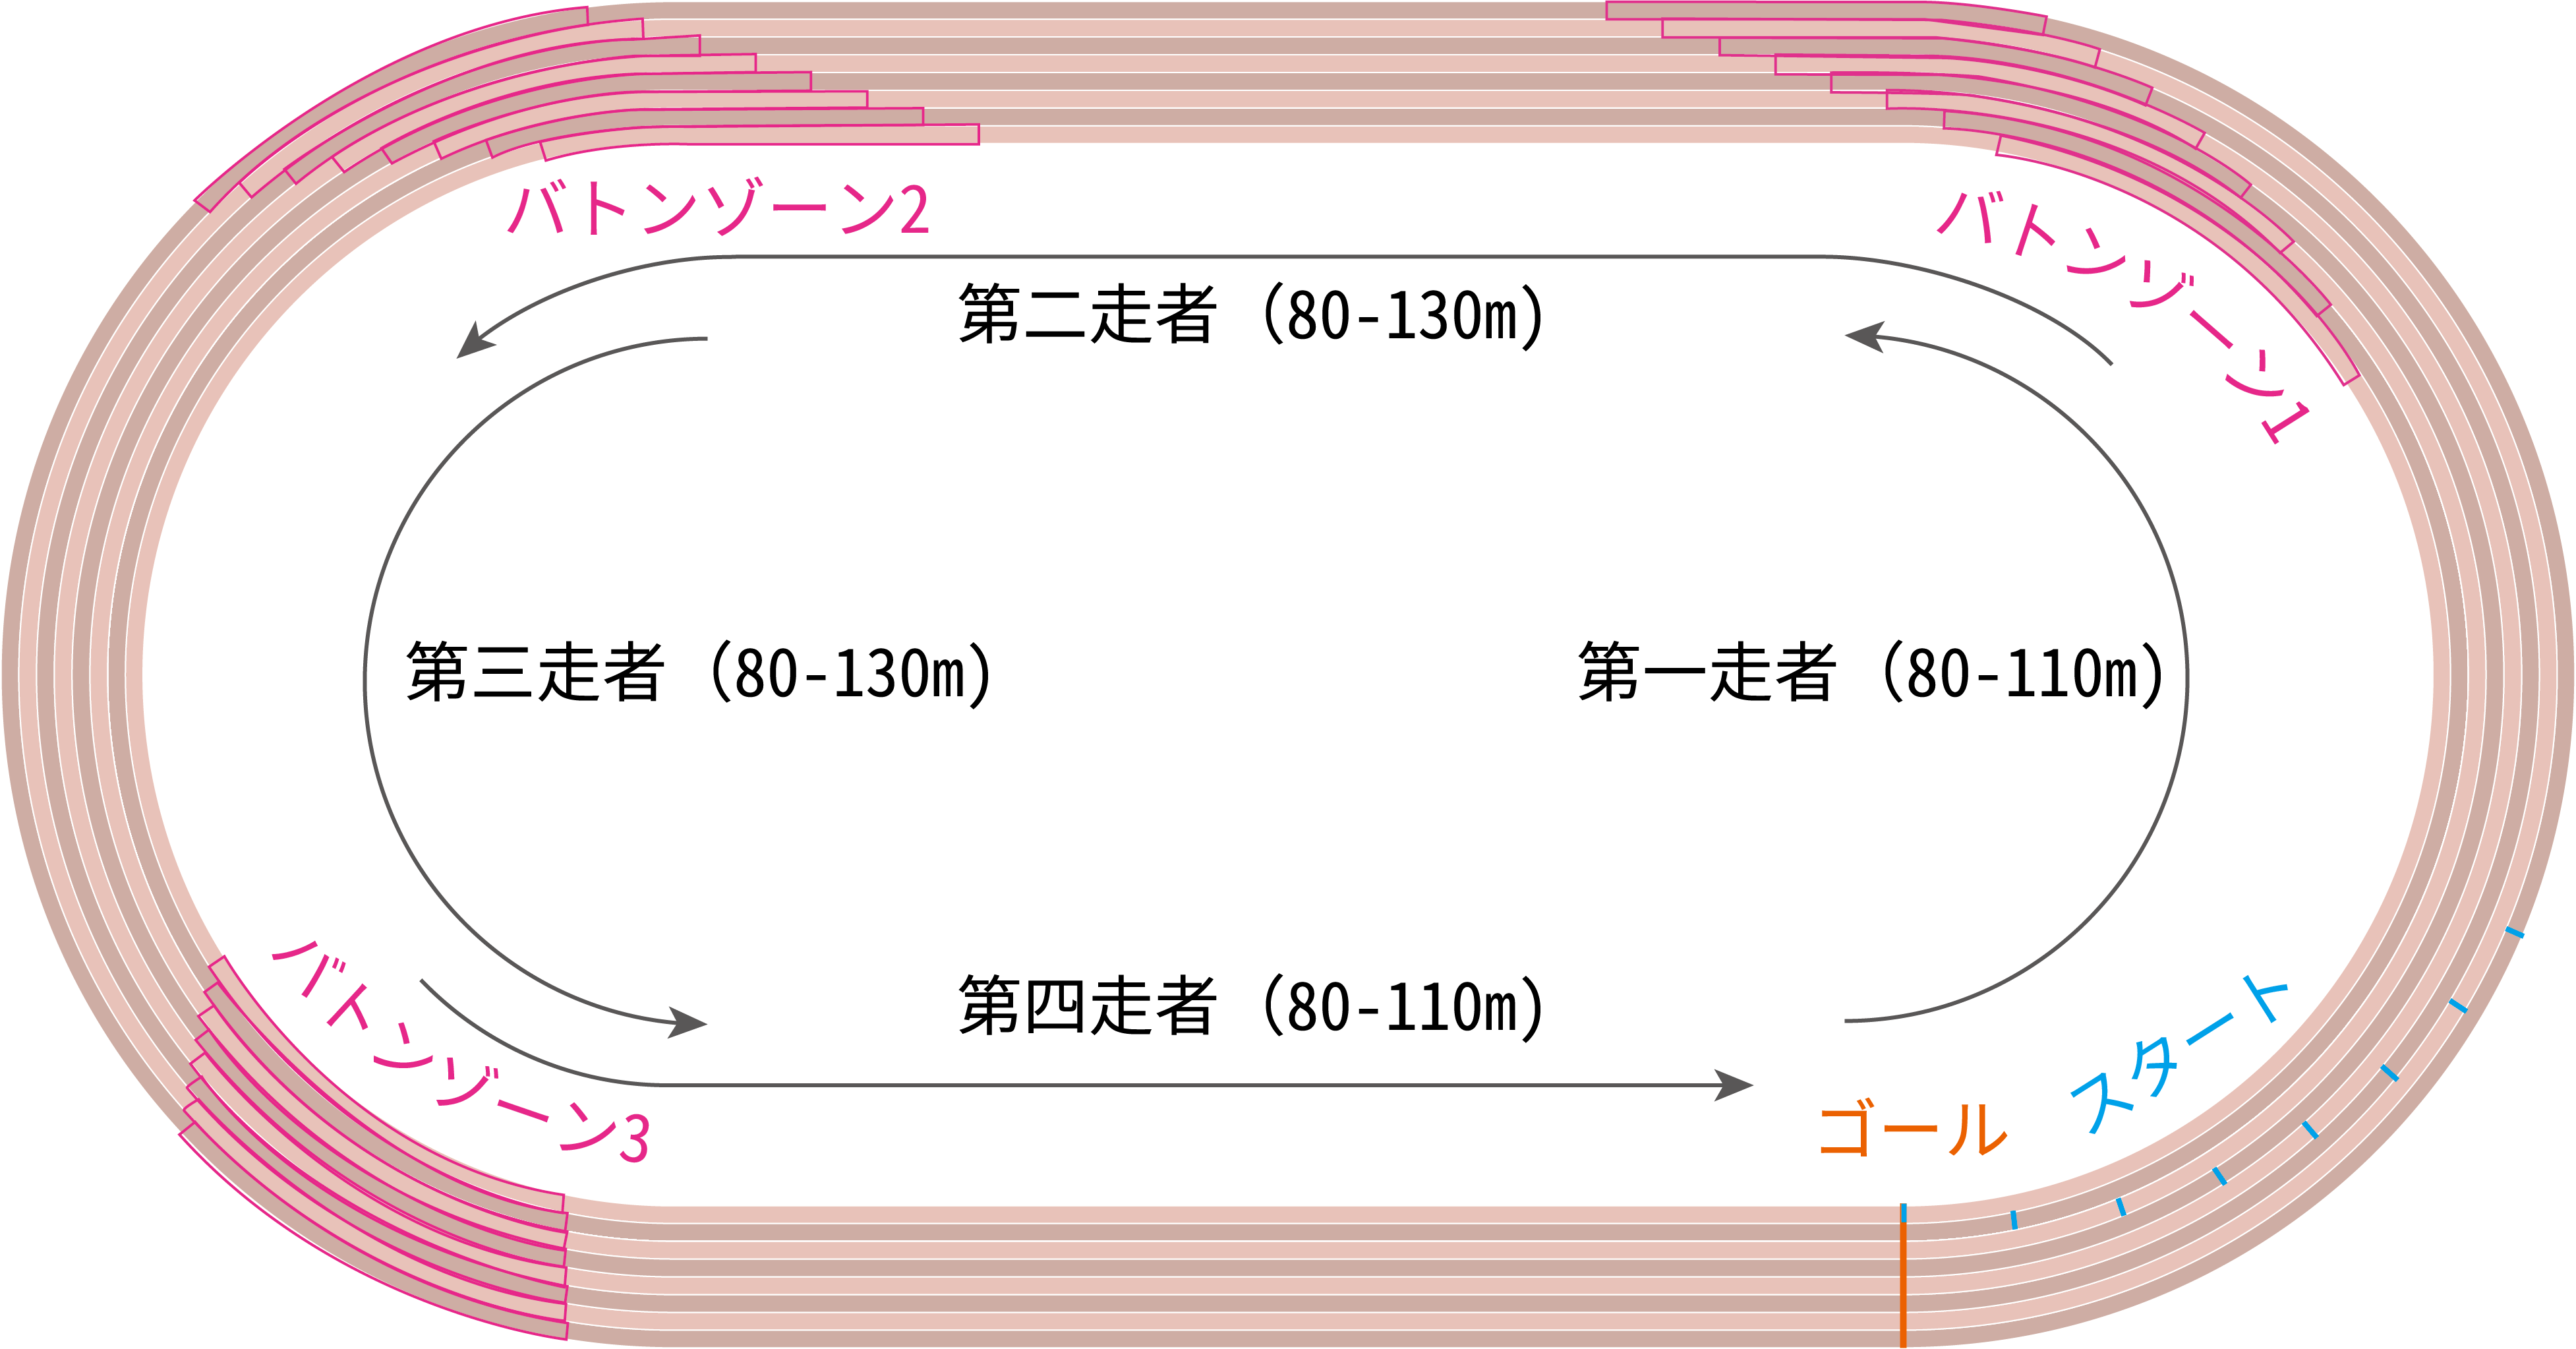
\includegraphics[width=0.7\textwidth]{../images/relay_2.eps}
\end{center}
\capwidth=90mm %
\caption{4×100mリレーの走路とバトンゾーン}
\label{fig:batonzone}
\end{figure*}

バトンパスは，現場のアスリートやコーチにとっても，奥深い技術である．
各バトンパスは，定められた30mのバトンゾーン内で完結させなければ失格となる．
バトンパスの巧拙/成否が記録を左右する．
世界大会の決勝ですら，バトンを落としたり受け渡しがゾーン内で間に合わなかったりして失格になることも少なくない．
逆に言えば，チーム4人の単体走力が低くとも，巧みなバトンパスによって相手チームに先着することもできる．
2016年リオオリンピック陸上男子リレー決勝
\footnote{
  動画はこちら．\url{https://www.youtube.com/watch?v=WaRRfc8GSZw}（2026年4月30日閲覧）
}がそれだ．
日本チームは，メンバー4人の100mシーズンベストタイムを単純合算した値だと，決勝8チーム中6番目に位置していた\cite{noguchi_online}．
だがそのビハインドを覆し，日本は銀メダルに輝いたのだ．

\subsection{リレーの既存研究}\label{subsec:prestudy_relay}

% 4×100mリレーにおけるバトンパス技術の研究は，ハイスピードカメラ等を用いた実証的な運動学的分析\cite{li2025}\cite{matsubayashi2022}\cite{zarebska2021}と，走速度プロファイルに基づいた数理的なシミュレーション研究\cite{karlsson2024}\cite{wardsmith2002}の両面から発展を遂げてきた．

リレーにおけるバトンパス技術の研究は，ハイスピードカメラ等を用いた実証的な運動学的分析\cite{li2025,matsubayashi2022,zarebska2021}と，\furu{}{走速度変化}に基づいた数理的なシミュレーション研究\cite{karlsson2024,wardsmith2002}の両面から発展を遂げてきた．

% 実証的研究においては，日本や中国，ポーランドのナショナルチームを対象として，バトンゾーン内でのバトンをもらう走者の加速度合いやバトンパス所要時間，バトンの差出しにともなう「利得時間」や「利得距離」といった指標がリレー走破タイムに関連する重要な変数として特定されている\cite{li2025,matsubayashi2022,zarebska2021}．
\furu{}{
実証的研究では，日本や中国，ポーランドの国内代表選手らを対象として，リレー時の走者位置・バトン位置が分析された．
その結果，バトンゾーン内での各走者の速度，バトンパス所要時間，バトンの差出し距離の大きさで得られる「利得時間」や「利得距離」といった指標がリレー走破タイムに関連する重要な変数として挙げられている\cite{li2025,matsubayashi2022,zarebska2021}．
}
数理的アプローチにおいては，\cite{wardsmith2002}による走速度や位置を主要な制御因子とした決定論的な最適化モデルがある．
近年では走者の走速度の不確実性を確率変数として組み込み，失格リスクと走破タイムのトレードオフを分析する確率的モデルも検討されている\cite{karlsson2024}．
このように，速度や位置，タイミングなど，バトン移動速度を最大化するための戦略的構造が明らかになりつつある．

上記のように，主に走者やバトンの位置・速度といった運動学的な変数でバトンパスは理解されてきたものの，いかにして変動の大きな環境の中でバトンパスを成立させているのか，その即興的・創造的知性に関する理解は不足している．
その知性システムを理解するためには，既存研究のような運動学的変数やその戦略構造のみならず，そもそもバトンパスがいかなるイベントの連なりとして成り立つ現象なのか，詳細に記述し，整備することが必要である．
% \subsection{目的と方法}\label{subsec:object_and_method}
% リレーという複雑系現象を理解するために，構成論的アプローチをとる．
% 構成論的アプローチ（ファイファー，池上先生，中島先生，）とは，ある現象に対して，その現象のモデルを構成することによって，XXXXある現象を実現するためのXXX．対象のメカニズムの解明とは違う．
% 論理学的に言えば，ある命題に対して，十分条件を示すのであり，必要条件を明らかにするものではない．
% 構成論的アプローチは，対象を観察・分析し記述する，という科学的方法とは相補的なものである．
% 複雑系で謎めいた現象に対して，対象メカニズムの解明に至らずとも，「明確化」することができるのが構成論的アプローチのひとつの意義である．

% 本研究では，現場の支援を重要視する．
% 研究者が理解するためにシステムを作る，というのみならず，現場の学習者が理解するためのシステムであり，ゲーム型にした．
% 構成論的アプローチでは通常，役にたつものが作られるわけではないが，ーーーーーーーーーーーー（中島先生，知能の物語）．

% 本研究の目的は，ーーーである．
% そのために本論文では，リレーバトンパスを表現するシステムをつくったシミュレーションということよりもむしろ，著者らがつくり，議論し，やってみて，という一連のプロセスを研究成果と考え，そうしたプロセスも適宜示すXXX．


\section{バトンパスをイベント系列化する}\label{sec:real}

\fix{}{
著者らは，バトンパスの動画をつぶさに観察したり，自身の経験を振り返ったりしながら議論を重ね，
バトンパスをイベント系列として分節・記述した（\ref{fig:batonpass}）．
% \ref{fig:batonpass}を本研究の一成果であると位置づける．
}

\ref{fig:batonpass}左側の連続写真は，\ref{subsec:what_is_relay}で触れた2016年リオオリンピックの男子リレー決勝の日本チームの第三・四走者間のバトンパスシーンを8局面に分けたものである
\footnote{
  2016年当時のルールでは，Rの出走位置は現行ルールと同じであったが，バトンゾーンは現行ルールのゾーン30mのうち後半20mだけであった（シビアだった）．
  だが本章の説明の本質部分に影響を及ばさないので，2016年の事例をもちいた．
}．
\ref{fig:batonpass}右側は，連続写真の各局面を，俯瞰視点でひとつのダイアグラムとして簡略表現したものである\footnote{
  「アキレスと亀」から着想を得た表現方法でもある．
}．
第三・四走者をそれぞれP，Rと表記している．
本稿では，バトンを渡す人をP，もらう人をRと略記する．
\ref{fig:batonpass}内では当該局面XのPとRの位置を「$PX$」の形で示している．
次段落で\ref{fig:batonpass}をもちいてバトンパスのシーンを説明する．
バトンパスの難しさを前面に出すために「生々しく描写」してみたい．
次段落の説明で（）内に書いた数字は，上記各局面を示す．

\begin{figure}[t]
\begin{center}
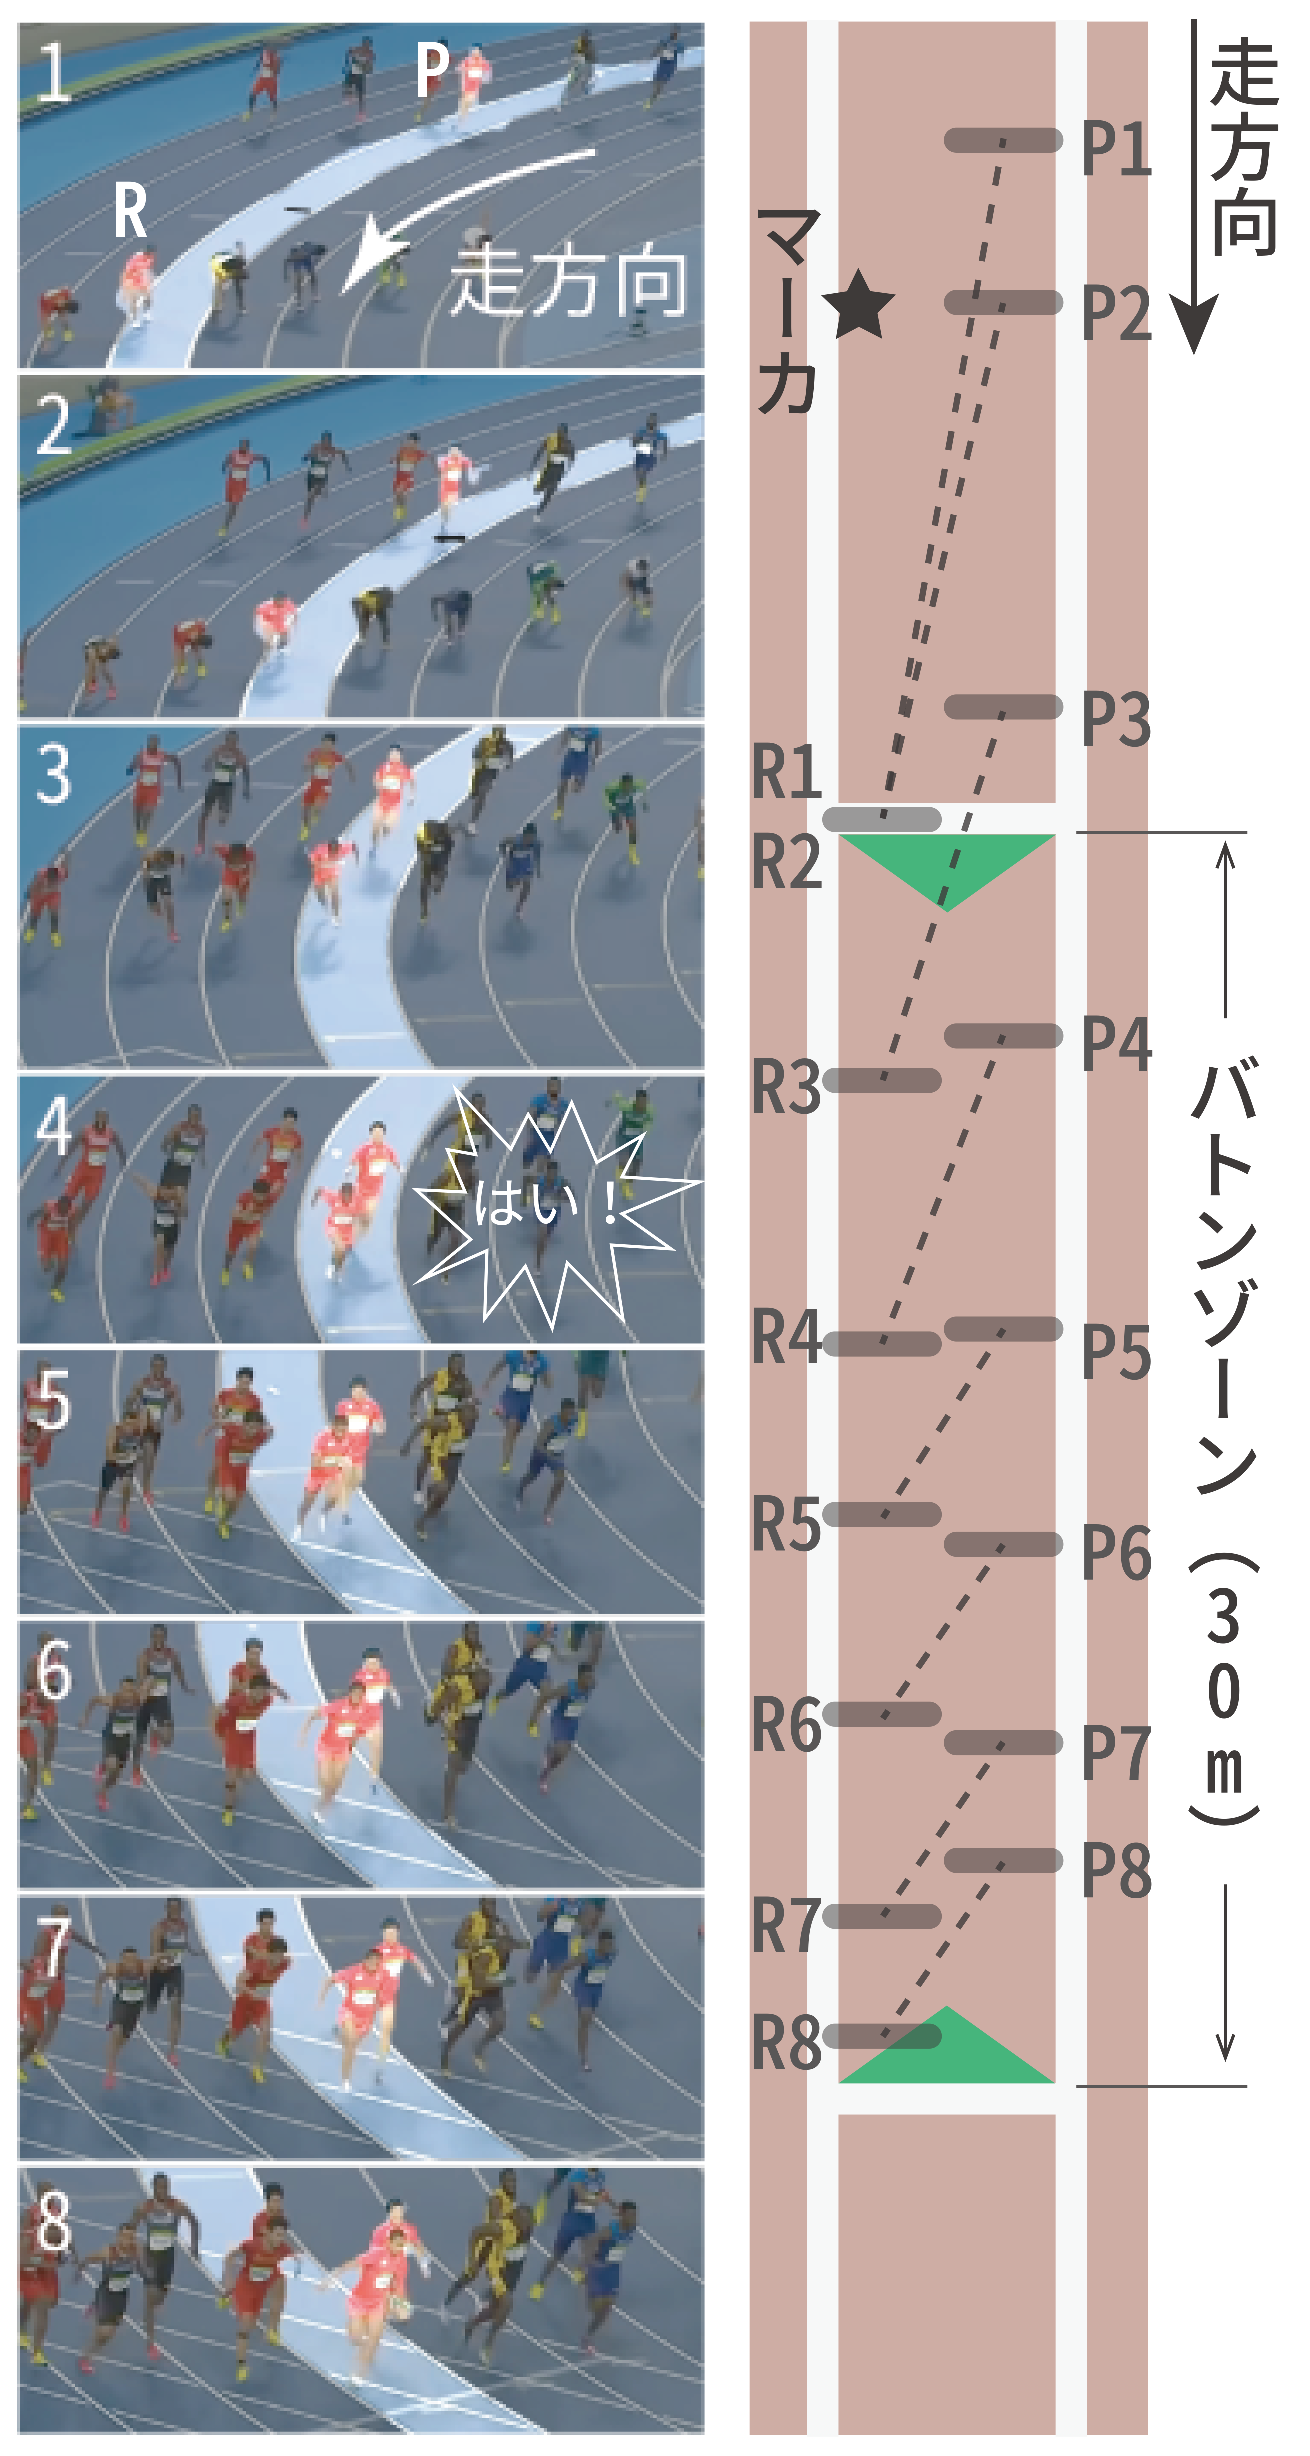
\includegraphics[width=\linewidth]{../images/baton_real_1.eps}
\end{center}
\capwidth=\textwidth %
\caption{バトンパスシーンのイベント系列（局面遷移）}
\label{fig:batonpass}
\end{figure}


Rはスタート姿勢をとりながら，Pが走ってくるのを観ている．
Pが高速で駆け込んでくる（1）．Pが「マーカ」（次段落参照）を通過する．
瞬間，Rは「今だ！」と思い切りスタートを切る（2）．
加速する．
後ろは振り返らない．
PがRに追いついてくる（3）．
PはRの背中に「はい！」と声で合図する（4）．
Rは振り返らずに，走りを維持しながらすぐさま左手だけ後ろに伸ばし，掌にバトンの感触がくるのを待ち受ける（5）．
すかさずPがバトンを差し出す．
Pの右手がRの左手にバトンを押し込む（6）．
Rが握る（7）．
Pが手離す（8）．
こうしてバトンが渡る．
わずか数秒のできごとである．

PとRのピッチや歩幅は毎回厳密に同じわけではない．
両者は高速状況下で互いの動きに即興的に応答しているのである．
両隣には相手チームも走っていることを忘れてはならない．
Rからすれば，Pを待ち構えているとき（\ref{fig:batonpass}の1〜2），むこうから8〜9人が一斉に雪崩こんでくる．
凄まじい勢いである
\footnote{
経験者である私（第一著者・堀内）は強く実感している．
また，陸上YouTuber「ケンちゃん」は「短距離走の恐怖の瞬間」のひとつとして，リレーにおいて第一走者が自分（第二走者）に駆け込んでくることを挙げている．
  \url{https://youtube.com/shorts/2tc2BrK8B10?si=zsga_FaetqDJKguV}．2026年4月30日閲覧．
}．
Rは「雪崩」のなかから「味方のエネルギー」をうまく感じとり，適切なタイミングで走りださねばならない．
そのためにPは適切位置にマーカを置いている．
だがマーカがあるにもかかわらず，焦って早く出たり，一歩目でバランスを崩して出だしが遅れることがある．
さらに言うならば，いつでもマーカ「だけ」を頼りに走り出すのがベストとも限らない．

もしもPがRに追いつきそうにないと判断したならば，Pはすかさず「待って！」と声をかける．
声を聞いたRが急減速することで，なんとかしてパスをつなぐ．
バトンゾーンをオーバーして失格になる事態だけは避けねばならないから，いたしかたないことなのだ．
また逆に，PがRに対して速すぎたならば，衝突を防ぐために，Pは減速せざるを得ない
\footnote{
  陸上界では俗に「バトンが詰まる」と表現する．
  「とりあえず予選レースを勝ち上がればよい」場合，あえてバトンを詰める「安全バトン」戦略をとることもある．
}．

とりわけ著者らが議論するなかで明確化したのは，バトンパス時にはRがPに追いつくだけではなくPとRの走速度がほぼ等しい必要があるという点や，
\fix{}{局面6・7・8の順序ある触覚的相互作用の存在である．}

以上のようにバトンパスは，高速かつ短時間で，全身をつかって，競争しながら協調して達成される．
しかも，視・聴・触覚が入り乱れたマルチモーダルなインタラクションとして成り立つ．
走者は互いの距離や速度，四肢の動きさえも「阿吽の呼吸」で調整するのである．
その場で即興的に創り出される身体的知性である．

では，こうしたインタラクションとしての知性は，システムとしてどのように表現可能になるのか？
著者らは，参照可能な概念を探った．

\section{参照概念}\label{sec:concepts}
生態心理学で環境との相互作用を記述する概念として扱われる「光学的情報$\tau$」と「位相$\phi$」に著者らは着眼した．
\subsection{光学的情報$\tau$（タウ）}\label{subsec:tau}
$\tau$とはなにか．
Leeら\cite{lee1982}は走幅跳を事例に$\tau$を実証的に説明した．
走幅跳選手は，数10m助走してきた勢いそのままに奥行きわずか20cmの踏切板を踏み当てることができる．
どうやって「歩幅調整」しているのか？

$\tau$とは，助走による移動にともない生じる光学的流動すなわち，網膜に映る踏切板像の膨張率\footnote{
網膜像の大きさの変化率に対する網膜像の大きさ$z/\dot{z}$であり，情報的には，対象までの接近速度に対する対象までの距離$x/v$に等しい．
}である．
$\tau$は「このままいくとあと何秒で踏切版に到達するか」（予測到達時間）という情報に等しい．
歩幅調整は$\tau$を絶えず知覚しそれに即応しさえすれば可能で，「踏切板までの距離と自身の速度」という情報を知る必要はない（計算論的にみれば$\tau$はそれら情報と等価である）のだとLeeは主張する
\footnote{
助走中の残り歩数Nは決まっているから，$τ$を$N$で割った「次の一歩に必要な空中時間」もわかる.
空中時間は接地の垂直インパルスで制御できる．
したがって，最後の数歩で接地の垂直インパルスを調整すれば，助走最後で踏切板を踏み当てられるというわけだ.
}．
$\tau$による歩幅調整はとくに助走最後の数歩で顕著に表れる．

またLee\cite{Lee1998}は，$\tau$の時間変化率$\dot{\tau}$にも着目している．
対象に向かって移動し到達直前で無理なく停止する（激しい衝突をすることなく，追いつく）ためには，
$\dot{\tau}$を$-0.5$以上で一定になるよう速度制御すればよいことを論じた（$\dot{\tau}=-1$で一定ならば，等速で接近してゆき衝突することを意味する）．


バトンパスにおいても$\tau$は，歩幅調整や声をかけるタイミングの判断といったことに関わると考えられる．


\subsection{位相}\label{subsec:phase}
近年，近接して走る者どうしの「個人間協調」の研究が動的システム理論の枠組みを中心に広がりを見せている．
そのなかで，周期運動としての走運動を振動子に見立てることで「位相（phase）」を計算する研究群がある．
\cite{varlet2015,furukawa2024}は，100m走の世界記録や日本記録が誕生したレース\footnote{
世界記録レース：\url{https://www.youtube.com/watch?v=DiJKCQSkjOw}

日本記録レース：\url{https://www.youtube.com/watch?v=0eyhH9RhRbI}

ともに2026年5月3日閲覧．
}
において，\furu{}{近接して走る2人のステップタイミングの相対的な位相関係を計算し，}同期現象を発見している．
\cite{varlet2015,furukawa2024}は個人間に生じる協調的作用がパフォーマンス（記録）に影響を及ぼす可能性も指摘している．

リレーを対象にしたこうした動的な位相関係の研究は依然としてみられないが，リレーのバトンパスは相手チームと競走しながらもPとRとで「協調」して達成する行為であることからも，位相の観点はバトンパスの記述に有用であろう．
パスはPとRが互いに対側の腕を同時に差し出して達成される．
これは「PとRの腕振りの位相関係」そのものである．


\section{制作したバトンパスシステム}\label{sec:tool}
著者らは，\ref{sec:real}\ref{sec:concepts}の内容を拠りどころにしながら，バトンパスを表現するシステムを制作した．
\subsection{システム概要}\label{subsec:overview_tool}

\begin{figure*}[t]
\begin{center}
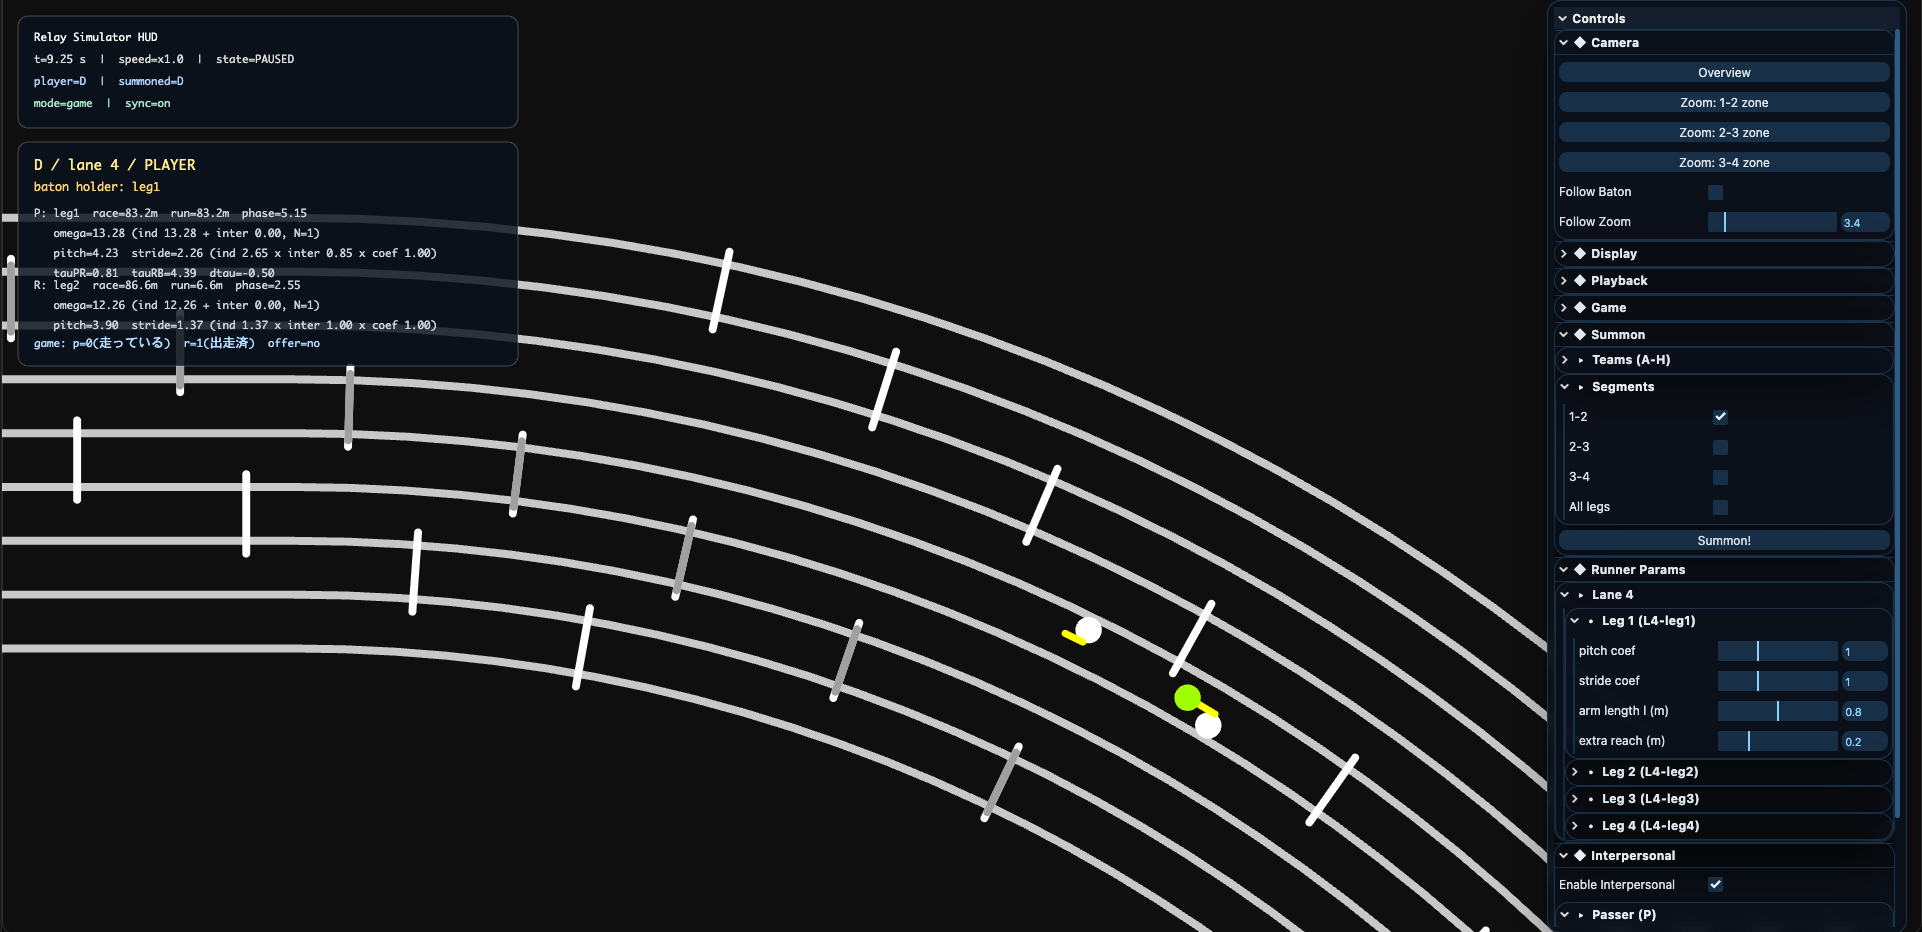
\includegraphics[width=0.7\textwidth]{../images/sim_overview.eps}
\end{center}
\capwidth=\linewidth %
\caption{システムの画面（左上はHUD，右側はGUIパネル）}
\label{fig:tool_overview}
\end{figure*}

バトンパスを体験するゲーム型システムとして設計した（\ref{fig:tool_overview}）．
システム（シミュレーション）を作ることをとおして知性を理解するというだけではなく，
現場のアスリートやコーチの学習を促すことをも目的に織り込んでいるからである．
webブラウザで動作する．
Javascript・HTML・CSSをもちいて開発しており，アニメーション部分にはp5.js，GUI部分にはlil-guiをもちいた．

陸上トラックを俯瞰する視点でリレーがアニメーションされる．
ユーザは俯瞰カメラの注視点移動とズームイン/アウトを操作できる．
\ref{fig:tool_overview}は，バトンゾーン1が映るよう，俯瞰カメラをズームインさせた状態である．
バトンゾーンは同レーン内の白線〜白線の区間であり，その間のグレー線はスタートから100m地点を表す．

4レーンの走者のみ示している．
走者は白い小円で表現される．
小円の端から，進行方向に伸縮する黄色い線が描かれ，これが腕（腕振り）を示す．
一・三走者は右腕，二・四走者は左腕のみ描かれる．
いずれもバトンを握るほうの腕である．
バトンは黄緑色の小円で描かれる．
走者のモデルについては\ref{subsec:runner_model}で述べる．

\ref{fig:tool_overview}は，\ref{sec:real}で示した局面2〜3に相当する．
右下の白線からRが走り出したのちにPがRとの距離を詰め，PR間距離が3.4mまで縮まった局面だ．
Pはバトンをもった右腕を前に振り切り，Rは左腕を前に振り込んでいる．

画面左上にHUD（Head Up Display）が表示され，\ref{table:hud1}・\ref{table:hud2}に示すとおり各変数の値が表示される．

% NOTE:HUD表１
% NOTE:HUD表１
\begin{table}[t]
\centering
\caption{HUDに表示されるシミュレーション全体の情報}
\label{table:hud1}
\small
\begin{tabularx}{\columnwidth}{lX}
\hline
項目 & 内容 \\
\hline
再生速度 & 現実時間に対するシミュレーション時間の比 \\
再生状態 & 再生 / 一時停止 \\
個人間相互作用成分の有無 & ピッチ・歩幅に対する相互作用成分の有無 \\
\hline
\end{tabularx}
\end{table}


% NOTE:HUD表2
% NOTE:HUD表2
\begin{table}[t]
\centering
\caption{HUDに表示される各走者の状態}
\label{table:hud2}
\small
\begin{tabularx}{\columnwidth}{lX}
\hline
項目 & 下位項目 \\
\hline

位置・運動状態
& 絶対位置・走破距離 \\
& 位相 $\phi$（\ref{subsubsec:oscillator}） \\
& 角速度 $\omega$（\ref{subsubsec:oscillator}） \\

\hline

ピッチ
& 個人内成分（\ref{subsubsec:intra_component}） \\
& 個人間相互作用成分（\ref{subsubsec:pitch_inter}） \\
& スケーリング係数（\ref{subsubsec:locomotion}） \\

\hline

歩幅
& 個人内成分（\ref{subsubsec:intra_component}） \\
& 個人間相互作用成分（\ref{subsubsec:length_inter}） \\
& スケーリング係数（\ref{subsubsec:locomotion}） \\

\hline

知覚情報
& 光学的情報タウ $\tau$（\ref{subsec:tau}） \\

\hline

局面情報
& 局面状態 \\

\hline
\end{tabularx}
\end{table}


画面右側にGUI（Graphical User Interface）が表示される．
GUIには\ref{tab:gui-items}で示す設定項目を設けた．


\begin{table}[t]
\footnotesize
\centering
\setlength{\tabcolsep}{3pt}
\renewcommand{\arraystretch}{1.08}
\caption{GUIパネルの項目一覧}
\label{tab:gui-items}
\begin{tabularx}{\columnwidth}{@{}p{0.20\columnwidth}p{0.32\columnwidth}X@{}}
\hline
\textbf{Section} & \textbf{Item} & \textbf{Description} \\
\hline
Controls & --- & GUI全体の最上位パネル．以下の各セクションを含む． \\
\hline
Camera & Overview & カメラを全景表示に戻す \\
Camera & Zoom: 1--2 zone & バトンゾーン1付近へズーム \\
Camera & Zoom: 2--3 zone & バトンゾーン2付近へズーム \\
Camera & Zoom: 3--4 zone & バトンゾーン3付近へズーム \\
Camera & Follow Baton & バトン追従カメラのON/OFF． \\
Camera & Follow Zoom & 追従時のズーム倍率を設定 \\
\hline
Display & Show HUD & HUD表示/非表示を切り替え \\
\hline
Playback & Speed (x0.1--1.0) & シミュレーション速度設定 \\
Playback & Restart Race (R) & 現在のGUI設定を保ったままレースをやり直す \\
\hline
Game & Enable Game & ゲームモードのON/OFF \\
\hline
Summon & Teams (A--H) $>$ Player Team & 操作対象となるプレイヤーチームを選ぶ\\
Summon & Teams (A--H) $>$ A--H & 召喚するチームを選ぶ\\
Summon & Segments $>$ 1--2 / 2--3 / 3--4 & 召喚する区間を選ぶ\\
Summon & Segments $>$ All legs & 全区間一括で召喚対象にする \\
Summon & Summon! & 選択したチーム・区間の走者を召喚する \\
\hline
Runner Params & Lane $n$ $>$ Leg $m$ & 走者ごとの個別設定 \\
Runner Params & pitch coef & 角速度（ピッチ）に掛かるスケーリング係数$\gamma$ \\
Runner Params & stride coef & ストライドに掛かるスケーリング係数$\gamma$\\
% Runner Params & start marker offset (m) & 非ゲームモード時のみ表示．第2走以降の出走マーカー位置を調整する． \\
Runner Params & arm length $l$ (m) & 腕長パラメータ．受け渡し可能距離の計算に関与\\
% Runner Params & extra reach (m) & 追加のリーチ量を設定する． \\
\hline
Interpersonal & Enable Interpersonal & 個人間相互作用成分のON/OFF\\
Interpersonal & Passer (P) $>$ Partners & Pが誰と同期するか\\
Interpersonal & Passer (P) $>$ Range (m) & Pの同期対象空間範囲\\
Interpersonal & Passer (P) $>$ K & Pの同期強度パラメータ\\
Interpersonal & Receiver (R) $>$ Partners & Rが誰と同期するか\\
Interpersonal & Receiver (R) $>$ Range (m) & Rの同期対象空間範囲\\
Interpersonal & Receiver (R) $>$ K & Rの同期強度パラメータ \\
\hline
\end{tabularx}
\end{table}


\subsection{走者のモデル}\label{subsec:runner_model}
本システムの特徴は，走者を「空間移動する振動子」としてモデル化する点である．
振動子は四肢の動きを表す．

\subsubsection{振動子モデル（位相）}\label{subsubsec:oscillator}
本研究では四肢は連動しているものとすることで，\ref{fig:phase}のとおり，ひとりの走者をひとつの振動子で表現する（つまり，\fix{}{現行システムでは}ひとりの走者の四肢間の相互作用については扱わない）．
腕振りの体側から体側までの「1往復」が，脚ステップの左足接地から次の左足接地までの「$2$歩」に相当し，
それらを振動子の1周期つまり$2π$[rad]に対応\furu{}{させる．}
腕振りを，この位相$\phi$の正弦$\sin\phi$をとることによって（それの時間変化としての）黄色伸縮線（\ref{subsec:overview_tool}）で表現する．
時間の流れにともなって振動子の位相が更新される．

\begin{figure}[t]
\begin{center}
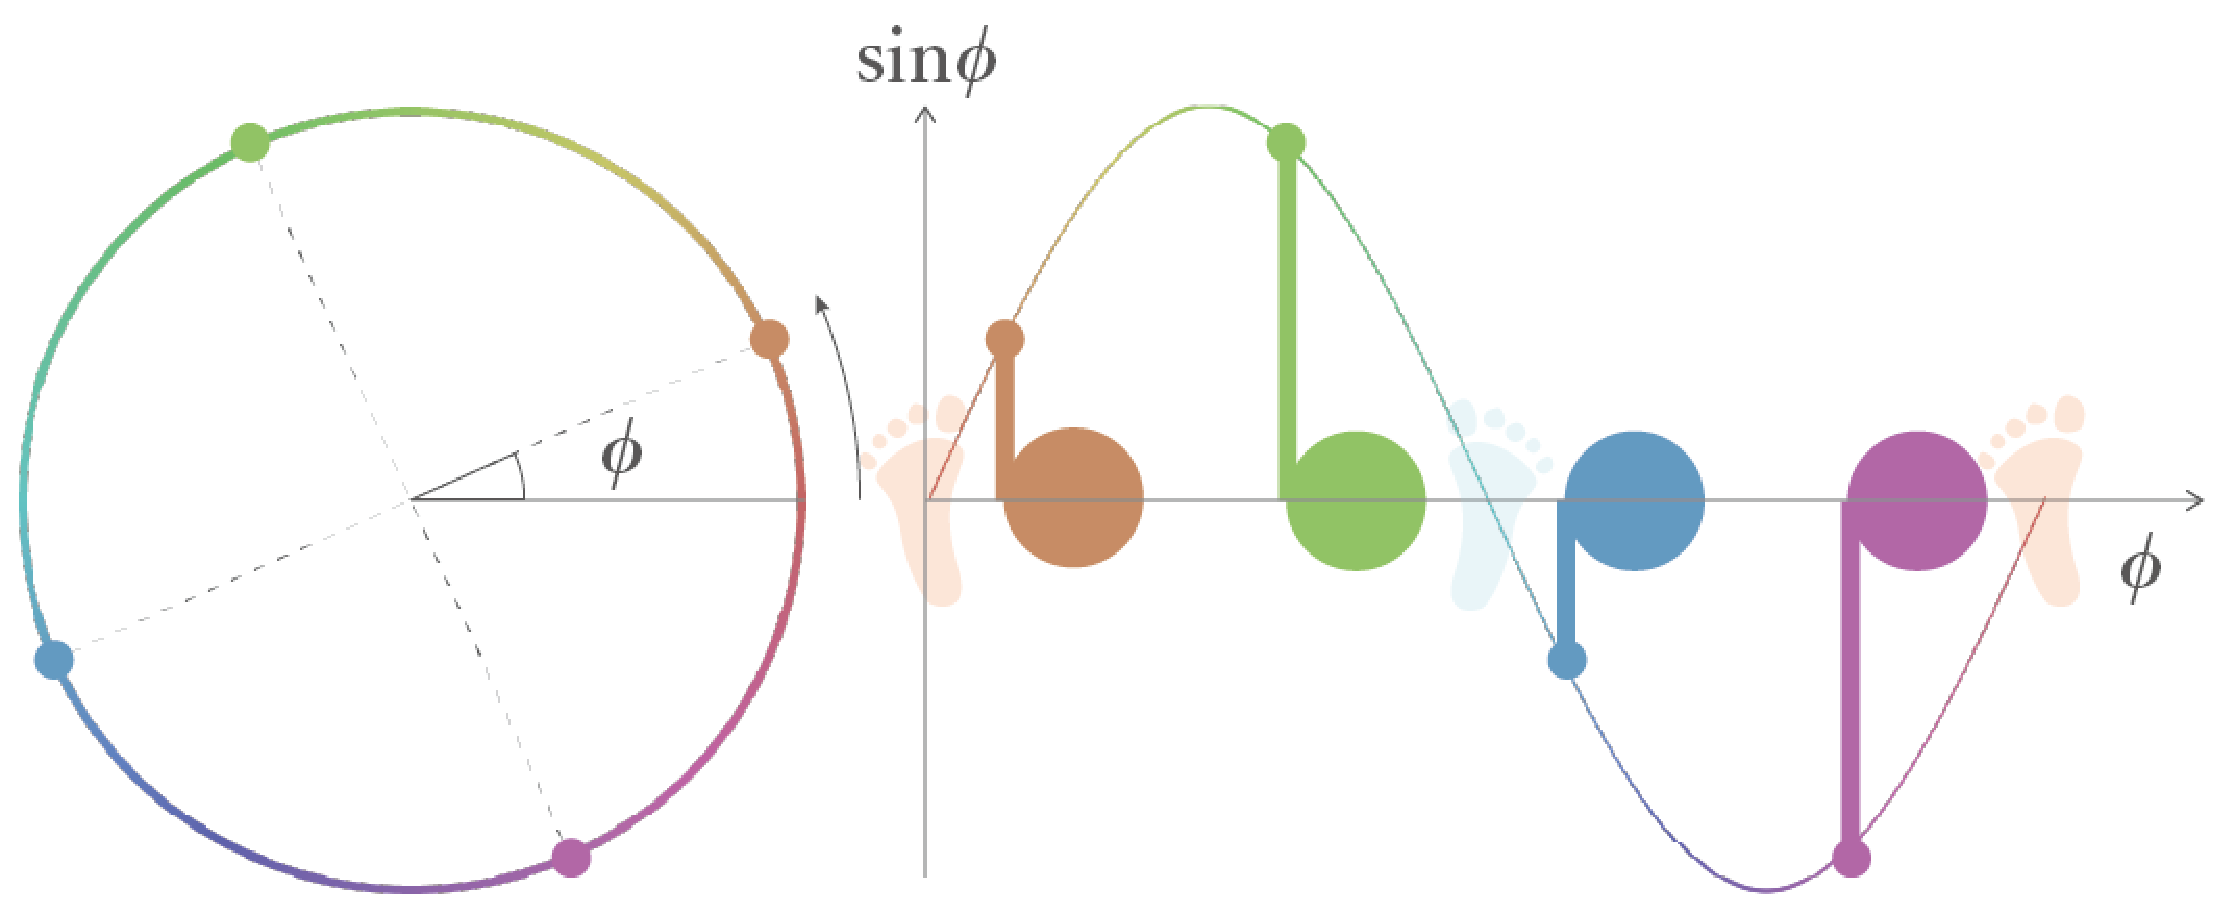
\includegraphics[width=\linewidth]{../images/graph.eps}
\end{center}
\capwidth=\textwidth %
\caption{走者の振動子モデル（$\phi$は位相）}
\label{fig:phase}
\end{figure}

\subsubsection{走者の空間移動（ピッチと歩幅）}\label{subsubsec:locomotion}
走者の空間移動も，位相をもとに定義する．
\fix{}{
走者の位置$x$[m]は走速度$v$[m/s]をもちいて式\ref{eq:x}のように更新する．
$\Delta t$はシミュレーション内部の時間最小単位であり，GUIパネルで設定する再生速度に応じて変化する．
\begin{equation}
  \label{eq:x}
  x(t+\Delta t) = x(t) + v \Delta t
\end{equation}
}
一般に$v$ [m/s] は，歩幅 $L$ [m] とピッチ $F$ [歩/s] をもちいて式\ref{eq:v}で表される．
\begin{equation}
  \label{eq:v}
\fix{}{v = F * L}
\end{equation}

ピッチ $F$ [歩/s]と振動子の位相速度（角速度）$\omega$ [rad/s] は比例する（式\ref{eq:pitch}）．
\begin{equation}
  \label{eq:pitch}
  F = \frac{1}{\pi}  \omega
\end{equation}


ピッチと歩幅はそれぞれ\fix{}{個人内成分（intra）}と個人間相互作用成分（inter）に分けて表現する（式\ref{eq:pitch_division}・\ref{eq:stride_division}）．
$\gamma$ はGUIのスライダで設定するスケーリング係数である．
\begin{equation}
  \label{eq:pitch_division}
F = (F^{intra} + F^{inter}) \gamma
\end{equation}

\begin{equation}
  \label{eq:stride_division}
L = L^{intra} L^{inter} \gamma
\end{equation}

\subsubsection{ピッチと歩幅の個人内成分}\label{subsubsec:intra_component}
個人内成分は本人の走破距離$x$を引数とする関数として定めた（式\ref{eq:pitch_intra}・\ref{eq:stride_intra}・\ref{table:pitch_coef}・\ref{table:stride_coef}・\ref{fig:pitch}・\ref{fig:stride}）．
これは，1991年世界陸上男子100m決勝レース8人の10mごとのピッチと歩幅のデータ\cite{ae1992} をもちいて，
その10mごとの8人の平均値を求め，その10点を3次スプライン曲線で補間することで連続関数化したものである．
100m以降は90-100mの変化を踏まえ外挿的に定義し，ピッチは一定値に指数関数的に収束させ，歩幅は一定値とした．

% NOTE:ピッチの個人内成分式
\begin{equation}
  \label{eq:pitch_intra}
F^{\mathrm{intra}}(x)=
\begin{cases}
\begin{aligned}
& a_k(x-x_k)^3 + b_k(x-x_k)^2 \\
& \quad + c_k(x-x_k) + d_k \\
& \text{for } x_k \le x < x_{k+1},
\end{aligned}\\
\begin{aligned}
& 4.20 + 0.25e^{-0.233(x-100)} \\
& \text{for } x>100,
\end{aligned}
\end{cases}
\end{equation}

% NOTE: 歩幅の個人内成分式
\begin{equation}
  \label{eq:stride_intra}
L^{\mathrm{intra}}(x)=
\begin{cases}
\begin{aligned}
& a_k(x-x_k)^3 + b_k(x-x_k)^2 \\
& \quad + c_k(x-x_k) + d_k \\
& \text{for } x_k \le x < x_{k+1},
\end{aligned}\\
\begin{aligned}
& 2.53 \\
& \text{for } x>100,
\end{aligned}
\end{cases}
\end{equation}

% NOTE:ピッチの個人内成分表
\begin{table}[t]
\centering
\small
\setlength{\tabcolsep}{3pt}
\renewcommand{\arraystretch}{0.95}
\caption{ピッチ関数 $F^{intra}(x)$ の係数}
\label{table:pitch_coef}
\begin{tabular}{ccrrrr}
  
\hline
$k$ & $x_k$ & $a_k$ & $b_k$ & $c_k$ & $d_k$ \\
\hline
1 & 10 & $-2.79{\times}10^{-4}$ & 0 & $1.01{\times}10^{-1}$ & 3.90 \\
2 & 20 & $3.62{\times}10^{-4}$ & $-8.38{\times}10^{-3}$ & $1.68{\times}10^{-2}$ & 4.63 \\
3 & 30 & $-4.40{\times}10^{-5}$ & $2.48{\times}10^{-3}$ & $-4.22{\times}10^{-2}$ & 4.38 \\
4 & 40 & $-4.61{\times}10^{-5}$ & $1.16{\times}10^{-3}$ & $-4.54{\times}10^{-2}$ & 4.52 \\
5 & 50 & $-2.77{\times}10^{-5}$ & $-2.23{\times}10^{-4}$ & $-3.60{\times}10^{-2}$ & 4.67 \\
6 & 60 & $8.33{\times}10^{-6}$ & $-1.06{\times}10^{-3}$ & $-4.88{\times}10^{-2}$ & 4.80 \\
7 & 70 & $4.44{\times}10^{-5}$ & $-8.05{\times}10^{-4}$ & $-6.74{\times}10^{-2}$ & 4.71 \\
8 & 80 & $-7.28{\times}10^{-6}$ & $5.27{\times}10^{-4}$ & $-7.02{\times}10^{-2}$ & 4.45 \\
9 & 90 & $-1.03{\times}10^{-5}$ & $3.09{\times}10^{-4}$ & $-6.14{\times}10^{-2}$ & 4.45 \\
\hline
\end{tabular}
\end{table}

% NOTE:歩幅の個人内成分表
\begin{table}[t]
\centering
\small
\setlength{\tabcolsep}{3pt}
\renewcommand{\arraystretch}{0.95}
\caption{歩幅関数 $L^{intra}(x)$ の係数}
\label{table:stride_coef}
\begin{tabular}{ccrrrr}
  
\hline
$k$ & $x_k$ & $a_k$ & $b_k$ & $c_k$ & $d_k$ \\
\hline
1 & 10 & $-4.88{\times}10^{-6}$ & 0 & $6.27{\times}10^{-2}$ & 1.37 \\
2 & 20 & $-7.44{\times}10^{-5}$ & $-1.46{\times}10^{-4}$ & $6.13{\times}10^{-2}$ & 1.92 \\
3 & 30 & $7.24{\times}10^{-5}$ & $-2.38{\times}10^{-3}$ & $3.60{\times}10^{-2}$ & 2.37 \\
4 & 40 & $-1.64{\times}10^{-5}$ & $-2.06{\times}10^{-4}$ & $1.02{\times}10^{-2}$ & 2.49 \\
5 & 50 & $4.93{\times}10^{-5}$ & $-6.97{\times}10^{-4}$ & $-1.08{\times}10^{-2}$ & 2.48 \\
6 & 60 & $1.00{\times}10^{-5}$ & $7.83{\times}10^{-4}$ & $-9.98{\times}10^{-3}$ & 2.40 \\
7 & 70 & $-3.64{\times}10^{-5}$ & $1.08{\times}10^{-3}$ & $8.68{\times}10^{-3}$ & 2.43 \\
8 & 80 & $3.27{\times}10^{-5}$ & $-7.31{\times}10^{-6}$ & $1.94{\times}10^{-2}$ & 2.59 \\
9 & 90 & $-3.25{\times}10^{-5}$ & $9.74{\times}10^{-4}$ & $2.91{\times}10^{-2}$ & 2.53 \\
\hline
\end{tabular}
\end{table}

% ピッチ関数グラフ
\begin{figure}[t]
\begin{center}
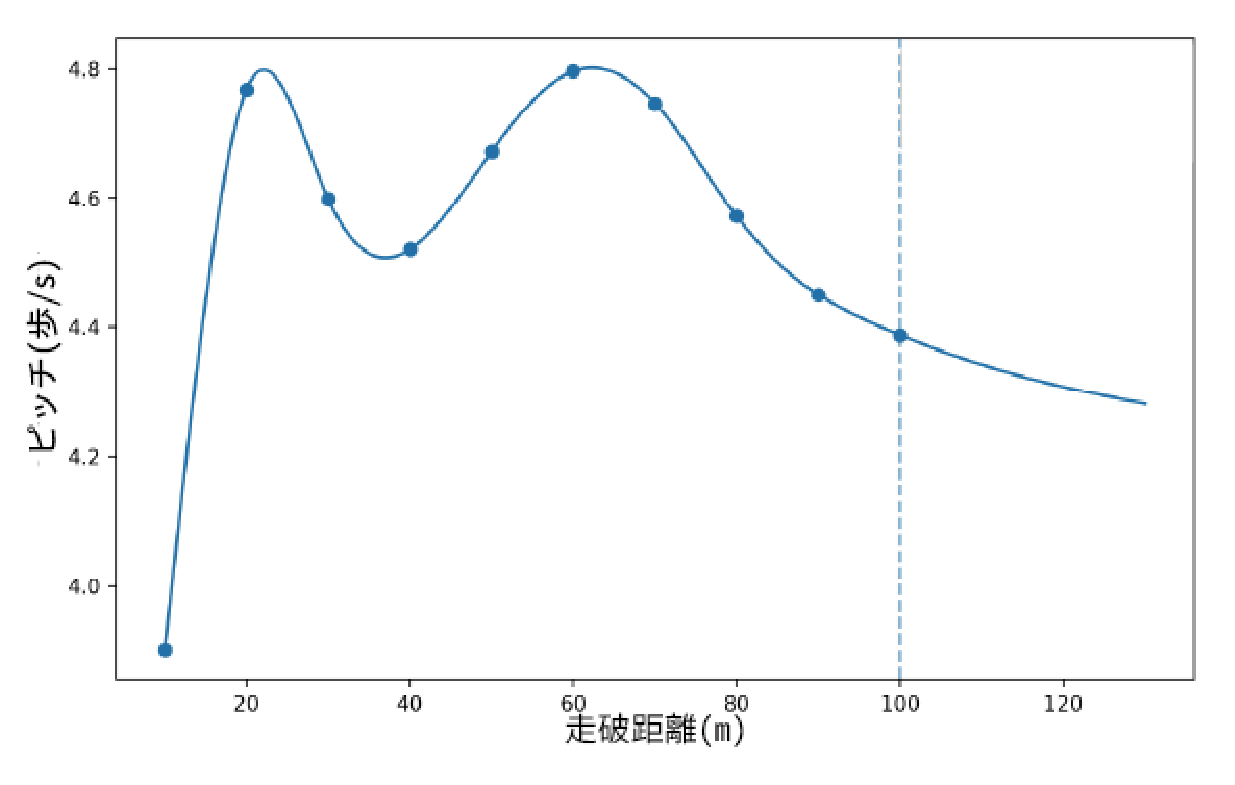
\includegraphics[width=\columnwidth]{../images/pitch.eps}
\end{center}
\capwidth=\textwidth %
\caption{ピッチの個人内成分$F^{intra}(x)$}
\label{fig:pitch}
\end{figure}

% 歩幅関数グラフ
\begin{figure}[t]
\begin{center}
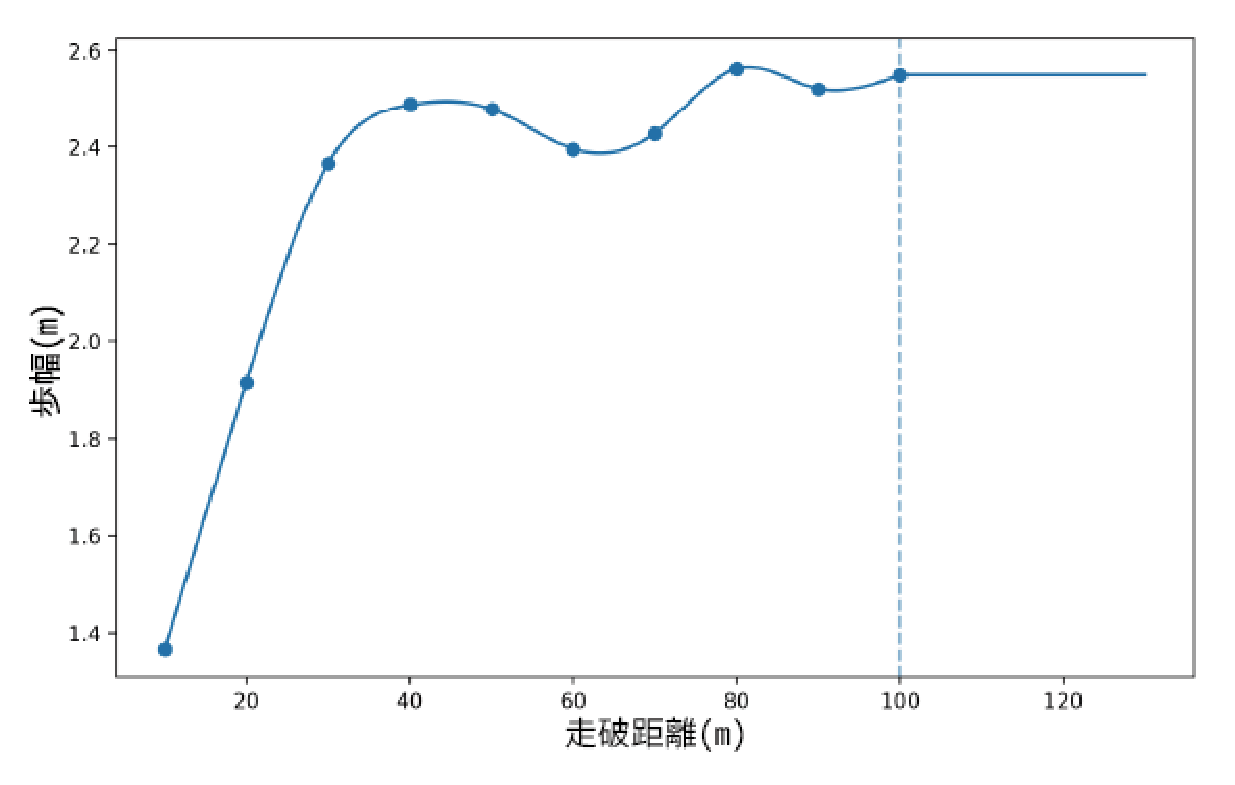
\includegraphics[width=\columnwidth]{../images/stride.eps}
\end{center}
\capwidth=\textwidth %
\caption{歩幅の個人内成分$L^{intra}(x)$}
\label{fig:stride}
\end{figure}
\subsubsection{ピッチの個人間相互作用成分}\label{subsubsec:pitch_inter}
ピッチの表現には，蔵本による結合振動子モデル\cite{kuramoto1975}をもちいた（式\ref{eq:oscilator}）．
ホタル群の明滅や同じ台に乗った複数のメトロノームの拍など，\furu{}{相互作用のある振動子群のふるまいを記述するモデルである．}
$K$は結合強度（同期の強さ），$N$は\furu{}{振動子}の数である．
\begin{equation}
  \label{eq:oscilator}
\frac{d\phi_i}{dt} = \omega_i + \frac{K}{N}\sum{\sin(\phi_j - \phi_i)}
\end{equation}

式\ref{eq:oscilator}はある時点の走者（振動子）$i$の位相速度を表し，
式\ref{eq:pitch_division}と同値である（両辺に$\pi$を乗じたもの．式\ref{eq:pitch}参照）．
ピッチの個人内成分は式\ref{eq:oscilator}の右辺第一項$\omega$に相当（比例）する．
したがって，ピッチの個人間相互作用成分は式\ref{eq:oscilator}右辺第二項に対応し，式\ref{eq:pitch_inter}で表せる．
\begin{equation}
  \label{eq:pitch_inter}
F^{inter} = \pi \frac{K}{N}\sum{\sin(\phi_j - \phi_i)}
\end{equation}

ユーザはGUIパネルから$K$と$N$を設定できる．
$N$は誰と同期するかという相手の範囲を選択する．

\fix{new!}{
システムにおいてPがRとピッチを同期させるようすを示す（\ref{fig:phase_transition}）．
Pのみ同期を設定し，$K=0.3$，$R$とのみ同期するようにした．
R出走直後（左一枚目）はほぼ同位相だったものが，6枚目ではほぼ逆位相になっているのがみてとれる．
}

\begin{figure}[t]
\begin{center}
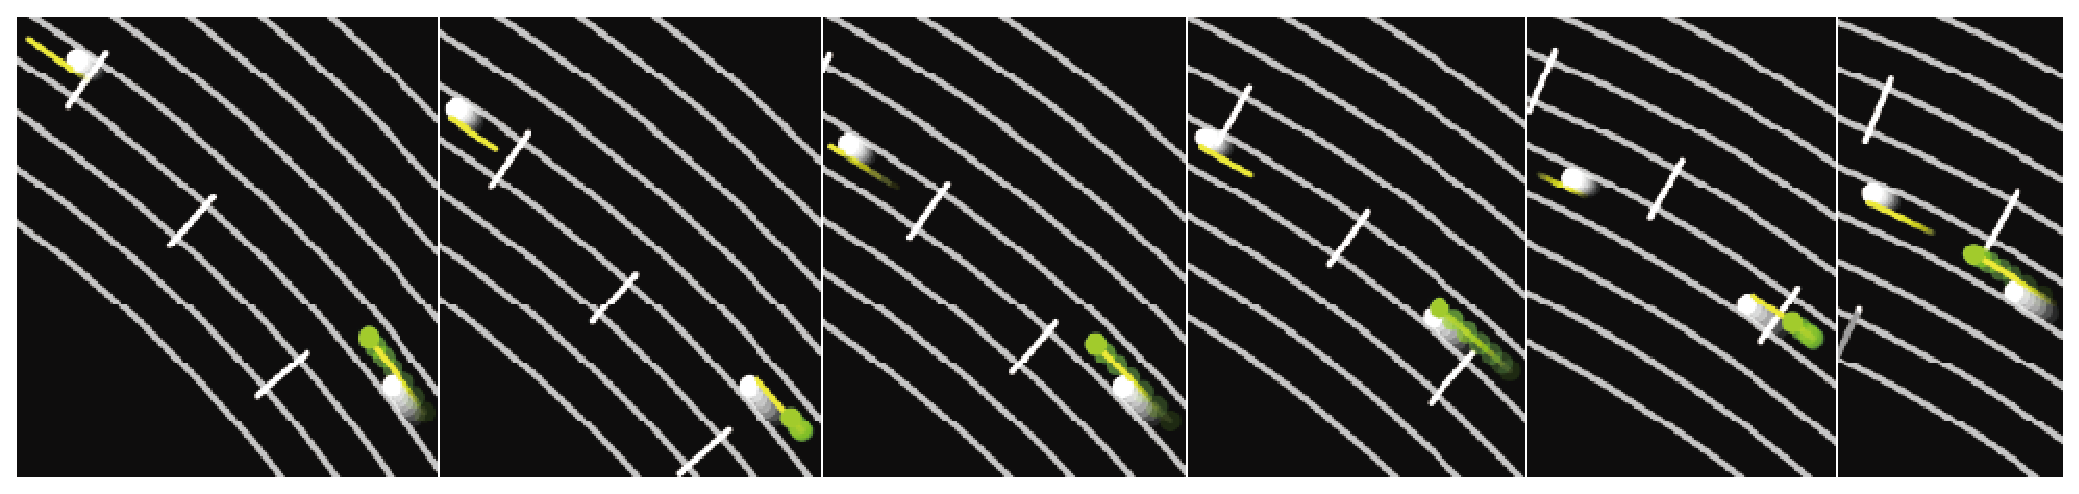
\includegraphics[width=\columnwidth]{../images/phase_transition.eps}
\end{center}
\capwidth=\textwidth %
\caption{PのピッチがRと同期するようす．（左画像から右画像へ）}
\label{fig:phase_transition}
\end{figure}


\subsubsection{歩幅の個人間相互作用成分}\label{subsubsec:length_inter}
\fix{}{
Leeらの研究を踏まえ，（\ref{subsec:tau}），歩幅の個人間相互作用成分には$\tau$の考え方をもちいた．
Pの歩幅個人間相互作用成分は，PがRに対して\furu{}{衝突}を避けるための滑らかな減速調整としてはたらく．
$\dot{\tau}_{PR}>=-0.5$で一定に保つような減速である．
まず，$\tau_{PR}$すなわちPがRに到達する予測時間は式\ref{eq:tau_pr}で表せる．
$x_R$と$x_P$はRとPの位置である．
}

\fix{}{
\begin{equation}
  \label{eq:tau_pr}
\tau_{PR} = \frac{x_R - x_P}{v_P - v_R}
\end{equation}
}
式\ref{eq:tau_pr}を時間微分し，Pの知覚する$\dot{\tau}_{PR}$を得る（式\ref{eq:taudot_PR}）．

\begin{equation}
\label{eq:taudot_PR}
\dot{\tau}_{PR} = -1 -\frac{(x_R - x_P)(a_P - a_R)}{(v_P - v_R)^2}
\end{equation}

aは加速度である．
PがRより速く（$v_P>v_R$），ある距離以内（$x_R-x_P <= D$）にいて，$\dot{\tau}_{PR} < -0.5$であれば，
Pは$\dot{\tau}_{PR} =-0.5$に近づくように歩幅$L^{inter}_P$を狭める，という歩幅調整をおこなう（式\ref{eq:stride_inter_P}）．
$M_{1}$はスケーリング係数である．

\begin{equation}
  \label{eq:stride_inter_P}
  L^{inter}_P(t+\Delta t) = L^{inter}_P(t) - M_{1} (-0.5-\dot{\tau}_{PR})
\end{equation}

システムの実例で説明する（\ref{fig:stride_sample}）．
$D=5$[m]，$M_{1}=0.01$に設定しており，どちらもPが69.9m地点にいるとき（8.00秒）にRは出走させている．
歩幅調整なし（上段）はで89.8m地点で追いつく（9.82秒）が，
歩幅調整あり（下段）では追いつくのが92.6m地点まで延びる（10.32秒），
このように歩幅調整が結果に効いてくる．

%歩幅調整のようす
\begin{figure}[t]
\begin{center}
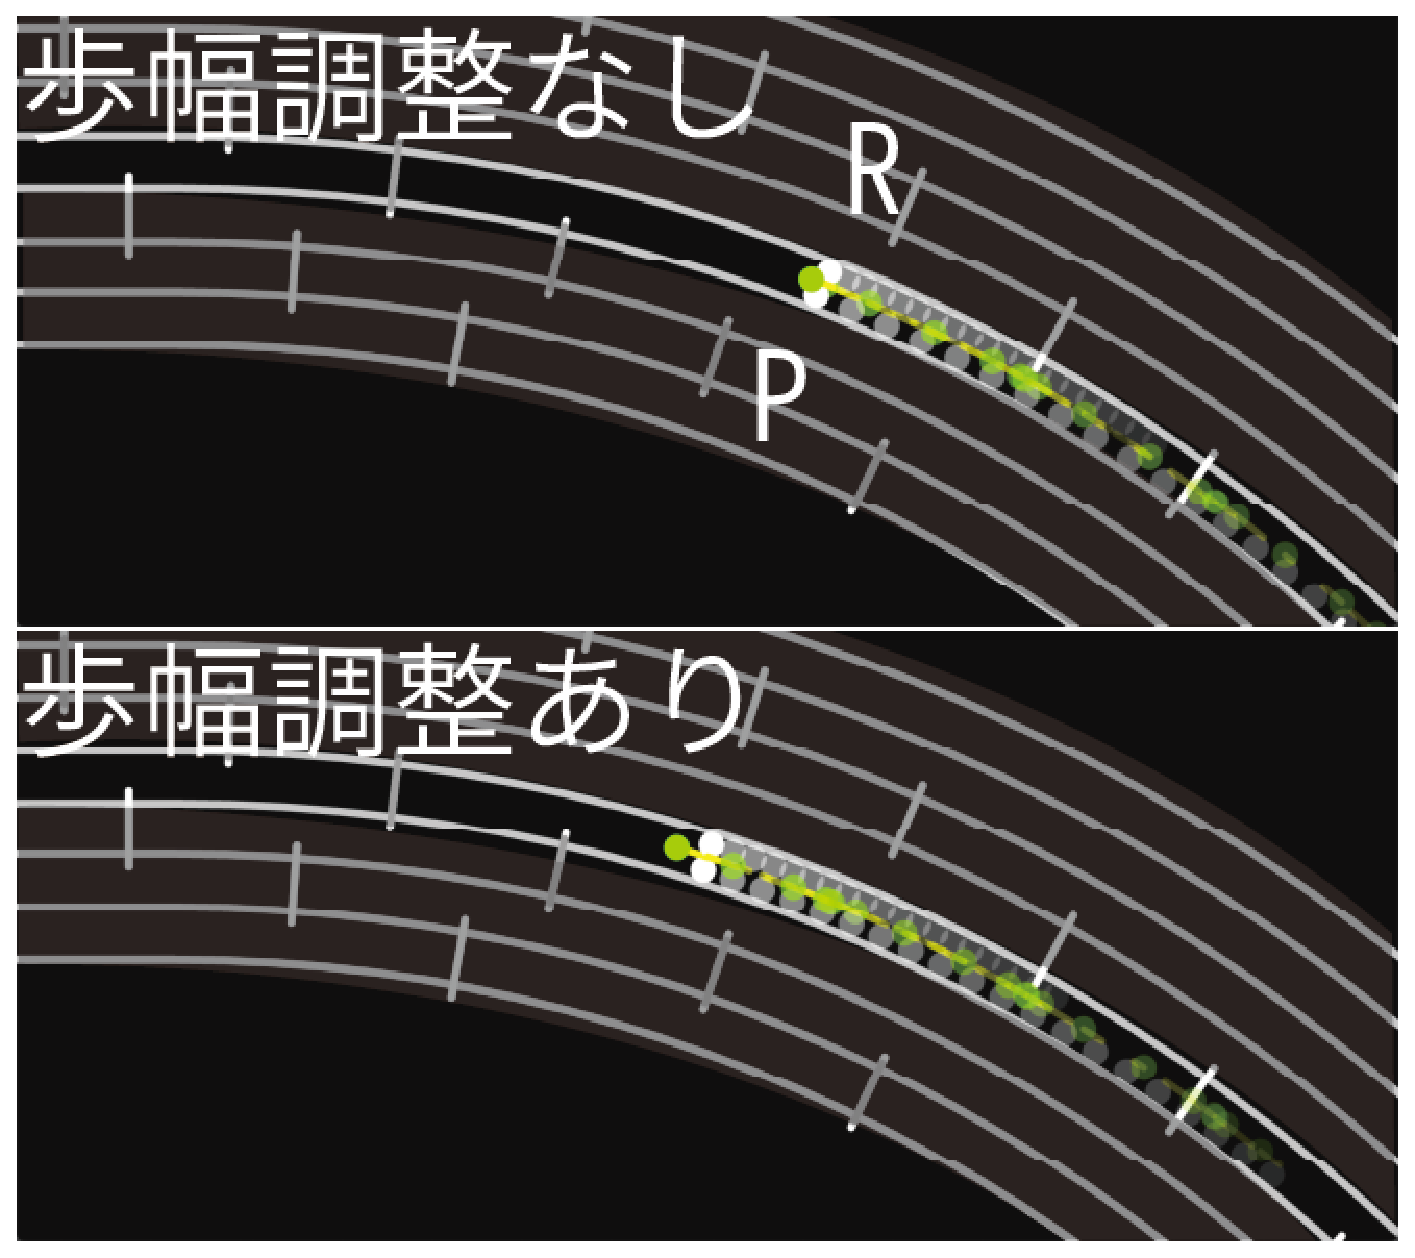
\includegraphics[width=0.7\columnwidth]{../images/stridesample.eps}
\end{center}
\capwidth=\textwidth %
\caption{Pの歩幅調整のようす（軌跡をつけて表示）}
\label{fig:stride_sample}
\end{figure}


また，Pが「このままだと，バトンパス前にRがゾーン終端に達する」と判断したならば，「待って!」と声かけしてRに減速してもらう．
この判断を，$\tau_{RB}$（式\ref{eq:tau_rb}）をもちいて，$\tau_{RB}$と$\tau_{PR}$の大小関係によって表現した（Pがこの関係性と等価な光学的流動を知覚している，と仮説）．
$\tau_{RB}$は，Rがバトンゾーン終端に到達する予測時間である．
$B$はバトンゾーン終端を表す．
\begin{equation}
  \label{eq:tau_rb}
\tau_{RB} = \frac{B - x_R}{v_R}
\end{equation}


「待って!」を聞いたRの歩幅個人間相互作用成分（減速）を式\ref{eq:stride_inter_R}で表す．
$M_{2}$はスケーリング係数である．
\begin{equation}
  \label{eq:stride_inter_R}
  L^{inter}_R(t+\Delta t) = L^{inter}_R(t) + M_{2} \dot{\tau}_{RB}
\end{equation}
\subsection{システムの操作方法}
ゲームでプレイするシナリオと方法を説明する．

\subsubsection{走者の召喚（GUIから操作）}\label{subsubsec:summon}
デフォルト状態では，4レーンの1・2走者のみ召喚されている．
GUIパネルより，参加チーム，第何走者を走らせるか，ユーザが操るチーム，を選択する．


\subsubsection{ゲームのプレイ方法}\label{subsubsec:play}
走者を召喚したのち，ゲームをプレイする．
ゲームは，走者のイベント系列（\ref{sec:real}）のかたちで進む．
プレイ中のキー操作一覧を\ref{table:key}に示す．
各イベントの実際のアニメーションと，その発生条件（局面遷移条件）を\ref{fig:game_phase}に示す．
ユーザは【space】キーを押して再生したのち，キーを押して走者PとRのアクションを制御する．

シミュレーションをベースにしたバトンパス体験型ゲームにするため，イベント発生条件には，ユーザのキー操作によるものと，そうでないものを設けた．
キー操作を発生条件とするイベントは，Rの出走(2)，Pの声かけ(4)，Rがバトンを握る(7)，Pがバトンを手離す(8)，の4つとした．
ユーザは，PとRのピッチと歩幅の変化様相（個人内/間成分）のなかで，PとRの上記2イベントずつをうまく制御する．
タイミングの学習を目論んだ．

イベント5と6の発生を自動にした理由は，走者にとって難易度の低いことだと判断したからである．
著者のリレー経験から，走者は5と6についてはイベント発生条件を意識しないままに，条件を満たしていたらほぼ自動的に遂行し，満たしていないと遂行しない（例えばPは，Rが遠くにいる状態でバトンを差し出すわけはない）．

しかしだからこそ，システムとしては，イベント発生条件を明確に記述することになった．
イベント5では，「はい!」を聞いたRが腕を後ろに伸ばして固定する．
これが起こるのは，走りの腕振りの流れのなかで，「はい!」の後に最初に腕を振り下ろしきった瞬間からである．
もし「はい!」の瞬間に「振り上げ中」の位相だったならば，そこから振り上げ切って再び振り下ろし，振り下ろし切った瞬間からようやくイベント5が発生するのであり，少なくとも，振り上げ位相から振り下ろし位相へ即座に移行できるわけではない（人間はそんな運動はできない）．

イベント6でPがバトンを差し出すにも，複雑な空間・時間的制約がある．
Rとの距離が十分近い必要がある．
Pの自然な走りのなかで，Rの手先までの距離をPの手先が届くぶんだけPが腕を振り込んだ瞬間である．
少なくともそれは，Pが走りのなかで腕を振り上げ中の位相でなければならない．
なお，パス時のPR間距離は，従来より「利得距離」\cite{matsubayashi2022}と呼ばれてきた変数である．

% 少なくとも，イベント5と6については，そういう明確化ができた（なお，イベント3はシステム上ではイベントとして扱っていない）．

Rがパス以前にバトンゾーンを超えたり，PがRに完全に追いつく（衝突）と，失敗となる（\ref{fig:failures}）．

\begin{table}[t]
\centering
\small
\caption{キーボードおよびマウス操作（[]内はキーを示す）}
\label{table:key}
\begin{tabular}{p{0.42\columnwidth} p{0.52\columnwidth}}
\hline
操作 & 内容 \\
\hline
【cmd】+マウスホイール（ピンチイン／アウト） & カメラのズームイン／アウト \\
【cmd】+ドラッグ & カメラ注視点の移動 \\
【space】 & アニメーション再生/一時停止\\
【ctrl】 & Rのアクション \\
【Enter】 & Pのアクション \\
【s】 & 再度スタート \\
【右矢印】 & コマ送り \\
【左矢印】 & コマ戻し \\
\hline
\end{tabular}
\end{table}


\begin{figure}[t]
\begin{center}
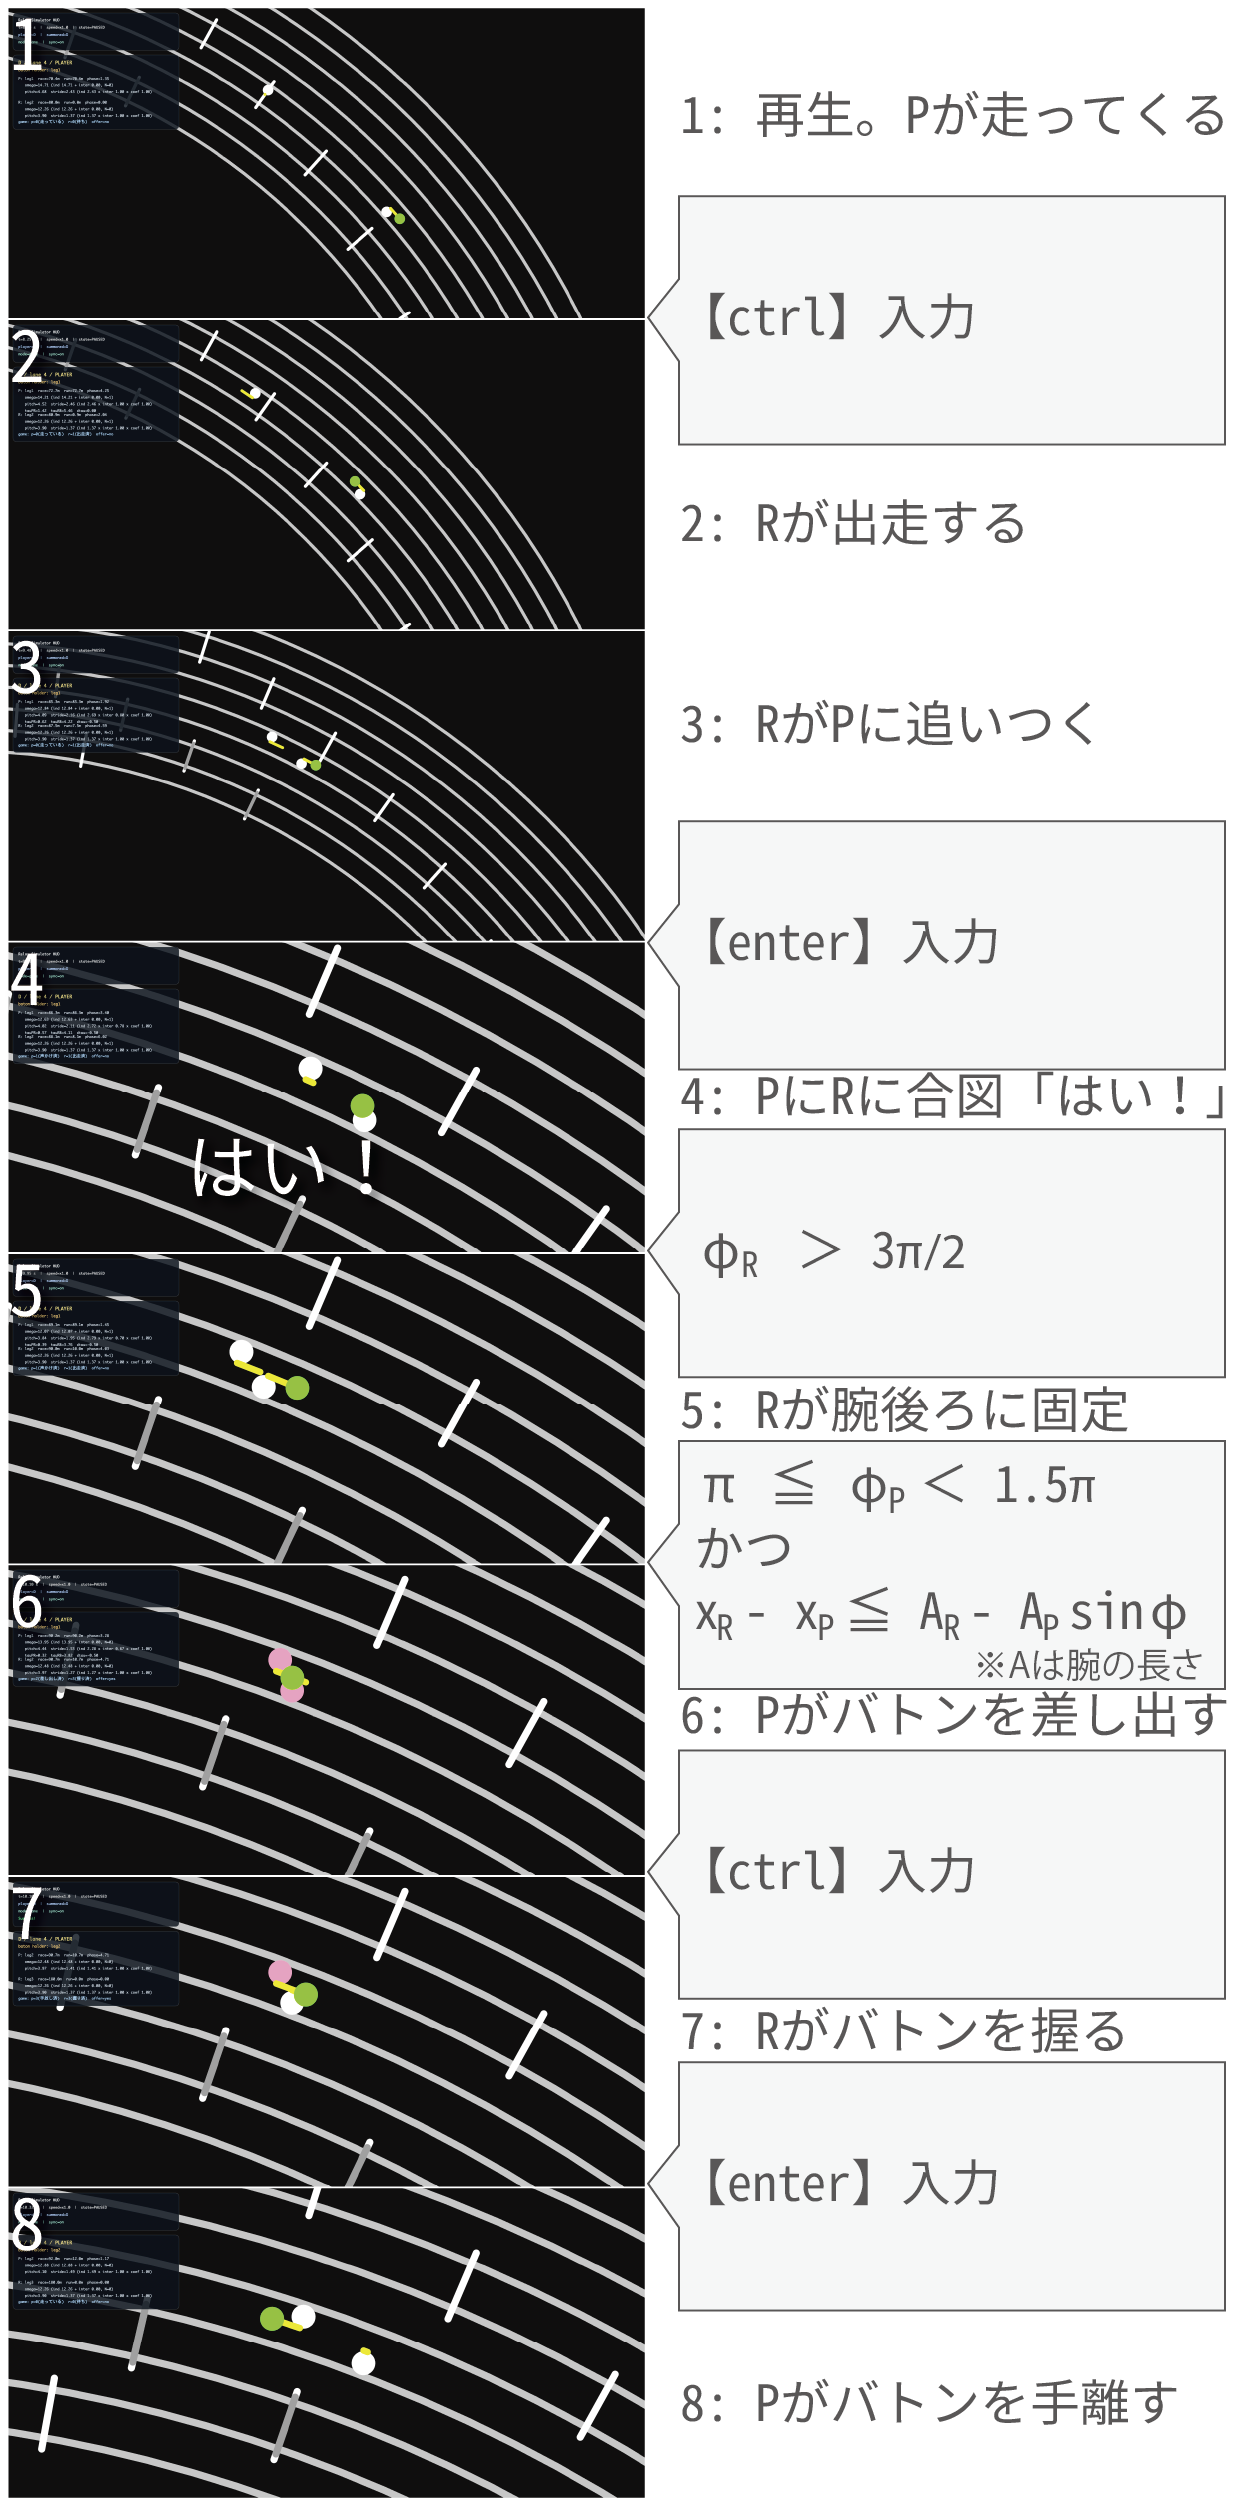
\includegraphics[width=\columnwidth]{../images/events.eps}
\end{center}
\capwidth=\textwidth %
\caption{各イベントのアニメーションと発生条件}
\label{fig:game_phase}
\end{figure}

%失敗のようす
\begin{figure}[t]
\begin{center}
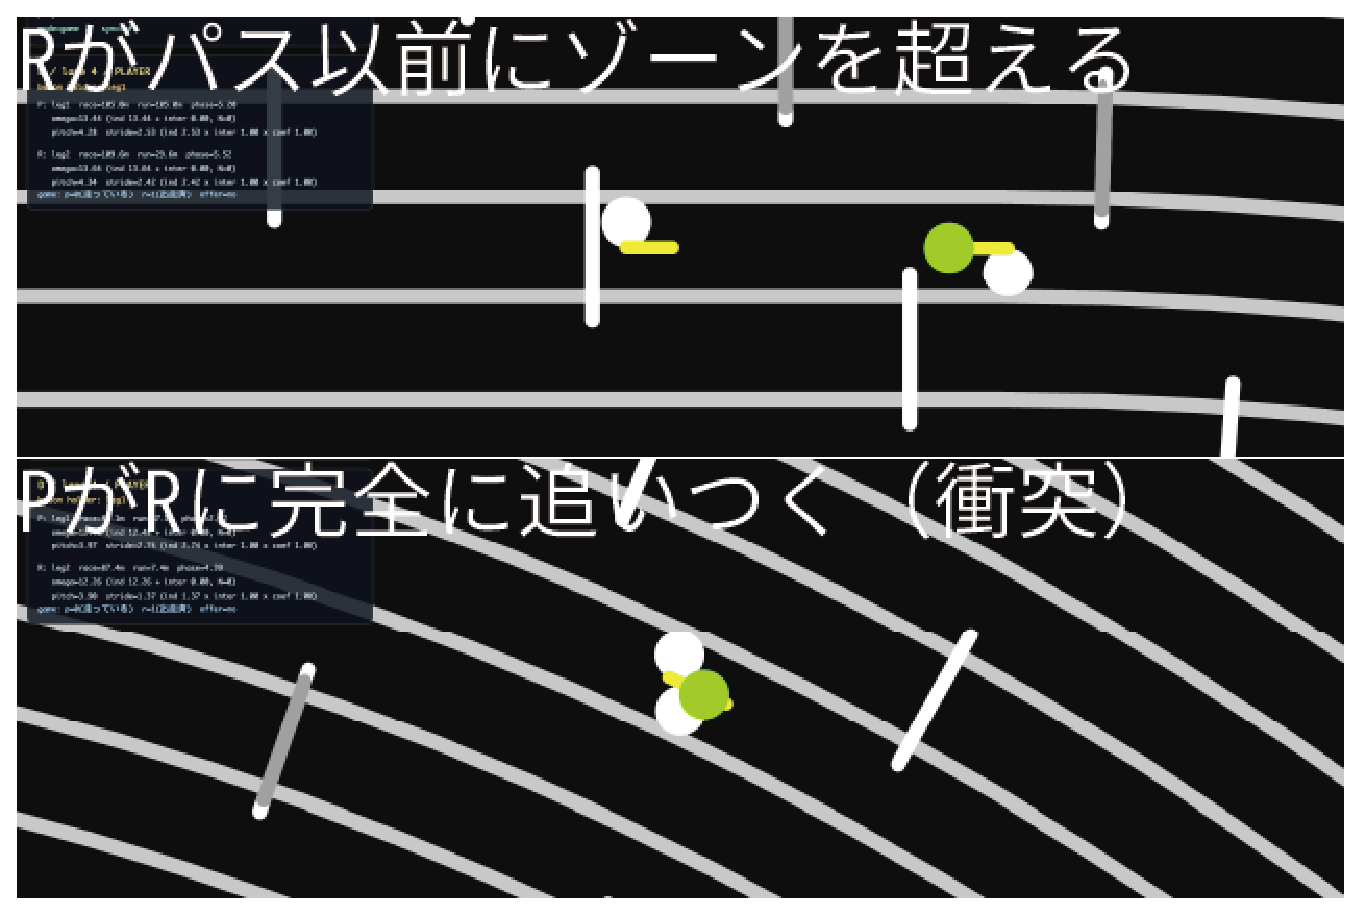
\includegraphics[width=0.7\columnwidth]{../images/failures.eps}
\end{center}
\capwidth=\textwidth %
\caption{バトンパス失敗パタン}
\label{fig:failures}
\end{figure}




\fix{}{
\section{システムを使ってみた}
}
\fix{}{
本システムを，異なる背景をもつ著者らで使ってみることで，バトンパス知性とそのシステムに関するさらなる気づきを探った．
プレイ方法を説明し，30分程度プレイし，互いに気づきを共有した（\ref{fig:comments_authors}）．
}

\begin{figure}[t]
\centering
\footnotesize
\setlength{\fboxsep}{4pt}
\ovalbox{%
\begin{minipage}{0.95\columnwidth}

\vspace{2mm}

\textbf{第一著者・堀内（陸上経験者，開発者）}
\begin{itemize}\setlength{\itemsep}{0pt}
  \item 実際のリレーでは自身がRとしてPを待ち構えるとき，Rとマーカの位置関係（その勢いを感じる自身の体感）に志向が支配されるけど，本システムでは鳥瞰的視点から眺めているからか，R出走以前から，「PとRとバトンゾーン終端との位置関係」を強く意識する．
  R出走キーを押す判断を，「今Rが出走すれば，バトンゾーン終端間際でPがRに到達しそうだ」といった見方が優勢になる感覚がある．
  このユーザとしての操作体験そのものは，システム内の走者の$\tau$の知覚モデルとはちがうモードな気がする．
  \item プレイ数をこなすうち，しだいに，Pの走るリズム（位相変化）に促されるようにR出走操作キーを押す感覚も生じた．
  \item 声かけタイミングは，Rが左腕を振り上げきった瞬間あたりで「はい!」と合図するのが良い
  \item ゲームだから何度も手軽にトライできる．
  \item GUIで個人間相互作用成分をOFFにすると，バトンパスは途端に難しくなる．容易にRがゾーンを超えたりPがRに衝突してしまう．．
  \item 自分ひとりでPとR二役を兼ねたゲーム操作は難しい．「二人プレイ」という仕様にするのも良いかもしれない．
\end{itemize}

\textbf{第二著者・古川（陸上経験者）}
\begin{itemize}\setlength{\itemsep}{0pt}
\item 「受け手をスタート，次は声掛けで，，」などと考えていたら間に合わない．順の想起などをせずに「タンタンタターン」という（ボタンタッピングの）リズムを「体得する」ほかないという感覚が，実際のリレーやその他の運動競技に似ている．
\item 現在のGUI（俯瞰的視点）だと，2者間の距離に応じた出発タイミングに主にほとんどの注意の認知資源が割かれる（腕振りの位置まで意識が回らない）．
\item 今回は走路を1次元に絞ってあり（進行方向に対して左右は考えなくてよい），その出発タイミングだけでも難しいのに，リアルではそれに加えて互いの手の位置を3次元的に一致させる必要がある．改めて認知的に高度な操作だと思った．
\item 実際の手の位相調整はどのようにされているのか改めて気になった．
\item 実際のリレー中，どのようなことに注意が向けられているのかを初心者から熟練者まで横断的に調査することで，実際のリレー練習に対してより効果的な実用的ツールへと改善していく指針を得られるであろう．
\end{itemize}

\textbf{第三著者・児玉（陸上未経験者）}
\begin{itemize}\setlength{\itemsep}{0pt}
\item リレー（バトンパス）そのものの理解が乏しいせいか，ゲームの操作やゴールの理解に難しさを感じた
\item R出走の「今だ」というタイミングがピンと来なかった（リレーをするという実体験や身体性の不足？）
\item PとRという2つの役割もピンと来なかった（それを俯瞰したユーザ視点でしか見れない感じ？）
\item 成功と失敗のフィードバックが弱いので，ピンと来なかった部分もあるかも？
\item 将来的には，コントローラが振動するなど，触覚的な情報もあると良いかも？
\item 走る「足音」や「はい！」「待って！」の掛け声も聴覚情報としてあると分かりやすくなる？
\item 背後でタウや位相同期のメカニズムが働いているなら，それを画面上に表示しちゃえば，タイミングの学習はしやすい？イメージとしては，タウ（ドット）の理想的な漸近線のグラフや，2つの振動子の相転移（同期）のグラフ？
\end{itemize}

\end{minipage}
}
\caption{著者らのシステム体験をとおした気づき}
\label{fig:comments_authors}
\end{figure}

\fix{}
{開発者である堀内は，アニメーションの俯瞰視点と実際のリレー時の視点の違いによる体験の違いや，
ゲームのほうが実際よりも手軽に「練習」できる点など，システム体験と実際のリレーとの違いに言及した．
リレー練習の大変さという現場課題に対して，手軽にシミュレーションできることはそれ自体価値がありそうである．
また，ひとりでPとRを兼ねることの難しさや，個人間相互作用成分のON/OFFの違いで難易度が変わることにも気づいた．
さらに，位相の観点から望ましいPの声かけタイミングや，Rの出走操作のタイミングなど，
システムをとおして実際のリレーの戦略や戦術につながる示唆を得た．
とくに後者については，Rは出走タイミングをはかる「マーカ」を，「Pとの距離」のみならず「Pの位相」をもうまく感得するためのものとして位置づけることができるのかもしれない．
そのように位相をも勘案した戦略の可能性が示唆される．
}

\fix{}{
古川は，走者を操作するリズムを身体でつかむことの重要性を指摘し，
俯瞰視点の限界の指摘，
パス時のPとRの手の三次元的位置と位相の調整という，実際のリレーが本システムのモデルよりも複雑であることを，システムをとおして認識したうえで．
本システムの実用性向上の方針を考えた．
}

\fix{}{
リレー体験をもたない児玉は，ゲームの操作やタスクおよびPとRの役割に「ピン」とこず，使用体験が難しかったことを述べている．
それに関連して，パスの成/否，マルチモーダル，システム内部状態（$\tau$や位相など）の明示など，
多様なフィードバックの強化の重要性について発想した．
}

\fix{}{
三人とも共通してゲームとしての難しさに言及しており，ゲームとしての設計には改良の余地があることが明らかとなった．
一般に，この手のシステムの開発や構築を行う工学的研究では，「つくる」までがゴールとされ，論文においても「つくったもの」の報告や記述が主となる．
いっぽう，本研究では「つくったもの」を「つかう」プロセスまでを研究の射程に入れ，構成的手法の範囲として扱う．
さらに，開発者・共同研究者（ユーザ）のバックグラウンドが少しずつ異なることで新たな気付きや発見が創発することがあると考え，あえて5章を設け，「つかってみた」プロセスの一端を掲載した．
}

\fix{}{
\section{展望}
}

\fix{}{
本研究は，リレーにおけるバトンパスの即興的で創造的な知性を，バトンパスをシミュレーションするゲーム型システムで表現した．
空間移動する振動子モデルによって走者を定義し，走者同士のインタラクションを$\tau$（歩幅調整）と位相（ピッチ調整）で定めたうえで，バトンパスを走者間で起こるイベント系列として記述した．
制作と実践を経て，リレー経験者として必ずしも自覚していなかったことがらも明確化された．
}


% 現場への還元拡張（CFP）
\fix{}{
本研究の限界と展望を述べる．
今後は，リレーの実践者（選手やコーチ）につかってもらうことで，現場の課題解決につなげたい．
そのために有効な現行システム改良点について述べる．
現行システムは，バトンパスを鳥瞰図的に眺める三人称視点でのアニメーションだが，バトンパス学習という意味では，一人称視点や二人称視点も重要であろう．一人称視点は，P視点ならばRを追いかける見え，R視点ならばPを待つ間は「雪崩」が迫ってきて，自身の出走後はPが視界に入らない見えである．
一人称視点はとくに$\tau$が直接関連し，実際のリレー時の見えに近い一人称視点は捨ておけない．
二人称視点は言わば「コーチの視点」である．
傍らからバトンパスを眺めるからこそ把握できるインタラクションの特徴があるかもしれない．
}

\fix{}{
現行システムで設計したユーザとのインタラクションは視覚的なものにとどまる．
聴覚的（「はい!」という発声や足音など）・触覚的インタラクションも実装したシステムという発展可能性がある．
たとえばタンジブルなバトン型インタフェースとし，振動で相手の位相をフィードバックするなどの工夫により，バトンパスの知性をより豊穣に体験できるシステムになるであろう．
}

\fix{}{
% 新しい指標の応用（CFP）
本研究では$\tau$と位相$\phi$というバトンパスに新しい変数（指標）を提案した．
$\tau$と位相が実際のリレー競技において利用されているか，また，今後の新しいバトンパス戦略として現実的に$\tau$と位相が活用できるか，という検証は今後の課題である．
}

\fix{}{
現場のデータ（練習や本番のリレー）をAIに学習させ，データ駆動型予測モデルの構築も可能である．
そのようにして，現場のアスリートや指導者が，本ゲームを実データやAI生成データとともにプレイすることで，さらにバトンパスの学習が促進される可能性がある．
}

\fix{}{
% フィジカルAI
バトンパスは，物体を二者間で受け渡す触覚的インタラクションに基づく協調的行為の一例として位置づけられる．
受け渡し行為の理解は，人とロボットのインタラクション（重い荷物の受け渡しや医療・介護の現場など）を扱うフィジカルAIの文脈においても重要である．
}

\fix{}{
本研究は，バトンパスをシミュレーション可能なシステムとして構成することを通じて，スポーツにおけるスキルの学習・習得支援のみならず，人と機械が物理的環境の中で協調するための知性を理解する手がかりを提示した．
今後，こうした知見が多様な実践領域へ展開されることを期待する．
}


\begin{acknowledgment}
%% 謝辞原稿の内容（省略）%%
\end{acknowledgment}

  \bibliography{btxsample}%%.bib ファイル名
  \bibliographystyle{jsai}%%jsai.bst スタイルの指定

% \begin{thebibliography}{??}
% \bibitem[]{}
% \bibitem[]{}
% \end{thebibliography}

% \appendix
% \section{付録}
%% 付録原稿の内容（省略）%%

\begin{biography}
\profile{正会員}{堀内隆仁}{2025年，慶應義塾大学大学院政策・メディア研究科後期博士課程単位取得退学，同年，博士（政策・メディア）取得．現在，東京都立大学客員研究員．身体知の学びの一人称研究，現象学的視点に立った身体知の学びの支援ツール，相互行為記述支援ツールの開発研究に従事．}
\profile{非会員}{古川大晃}{2019年熊本大学教育学部生涯スポーツ福祉課程卒業．2021年九州大学大学院人間環境学府行動システム専攻修士課程修了．2025年東京大学大学院総合文化研究科広域科学専攻博士課程修了．2025年から現在まで日本学術振興会特別研究員および京都工芸繊維大学情報工学・人間科学系特任助教を務める．走運動における認知，個人間の相互作用，集団形成のダイナミクス，集団走の効果に関する研究に従事．日本体育・スポーツ・健康学会，ランニング学会会員．博士（学術）．}
\profile{正会員}{児玉謙太郎}{2014年，総合研究大学院大学情報学専攻博士課程単位取得退学，神奈川大学特任助教．2015年，博士（情報学）取得． 2017年，同大学特任准教授．2020年，東京都立大学准教授．身体運動，知覚，コミュニケーションに関する研究に従事．}

\end{biography}

\end{document}

\subsubsection{\texttt{Vol}と\texttt{No}}\label{Vol}
\ltt{Vol} には \verb/\Vol{15}/ のように巻数（1985年が第1巻）を指定します．
\verb/\No/ は \verb/\No{1}/ のように号数を指定します．
論文が採録されて，掲載号が通知されたのち正しい巻と号を指定します．
よって，投稿時には指定しなくても問題ありません．

\subsubsection{\texttt{SubNo}}
論文番号を指定しますが，これは事務局が決定するため，指示がなければ
何もしなくて結構です．

\subsubsection{\texttt{jtitle}}
日本語タイトルを書きます．
タイトル中に改行（\verb|\\|）を指定すれば，タイトル中で改行できま
すが，柱\footnote{ヘッダ．ページ上部のページ数などがある部分}
では無視されます．長すぎて，柱に収まらない場合は，
\begin{verbfbox}
\jtitle[柱用タイトル]{タイトル}
\end{verbfbox}
\noindent
のようにすれば，柱には\verb|[]|内のものが使われます．

\subsubsection{\texttt{etitle}}
英語タイトルを書きます．
前置詞，接続詞，文中冠詞等を除き単語の先頭文字を大文字にします．

\subsubsection{\texttt{jsubtitle}と\texttt{esubtitle}}
サブタイトルがある場合は，これらを用いて指定します．
\verb/\jsubtitle/ は日本語用，\verb/\esubtitle/ は英語用です．
これらは柱には出力されません．

\subsubsection{\texttt{author}，\texttt{name}，\texttt{affiliation}}

著者のリストを，以下のように指定します．
\begin{verbfbox}
\author{%
 \name{姓}{名}{ローマ字読み}
 \affiliation{日所属}{英所属}{e-mail,URL}
}
\end{verbfbox}

\bsl{name} の第1引数は著者の姓を，第2引数は名を指定します．
第3引数は著者のローマ字名を指定します．
また，名前が長い方は\verb/\name/の代わりに
\verb/\longname/を使ってください．

著者の所属などは \verb/\affiliation/ に
指定します．
第1引数は著者の日本語所属名を，第2引数は英語所属名を
指定します．
第3引数は著者のe-mailアドレスを指定し，ホームページがあれば，``,''に続けて
そのあとにURLを記してください．URL中の``\~{}'' はそのまま（エスケープしな
いで）書いて下さい．

\subsubsection*{複数の著者の場合}

複数の著者の場合は\verb|\and| を使用します．
\begin{verbfbox}
\author{%
 \name{姓1}{名1}{ローマ字読み1}
 \affiliation{日所属1}{英所属1}{e-mail,URL}
\and
 \name{姓2}{名2}{ローマ字読み2}
 \sameaffiliation{e-mail,URL}
\and
 \longname{姓3}{名3}{ローマ字読み3}
 \affiliation{日所属3}{英所属3}{e-mail,URL}
\and
 \longname{姓4}{名4}{ローマ字読み4}
 \affiliation{日所属1}{英所属1}{e-mail,URL}
}
\end{verbfbox}
\noindent
同じ所属の著者が連続する場合は\verb/\affiliation/の代わりに
\verb/\sameaffiliation/を利用して，メールアドレスとURLだけを記述して
ください．上の例では，著者1と2は所属が同じため著者2の所属は
\verb/\sameaffiliation/を利用します．
ただし，同じ所属でも，連続していない場合は\verb/\affiliation/を用
いています．
著者4は著者1と所属が同じですが，間の著者3の所属が異なるため
\verb/\affiliation/を利用します．

著者が多い場合（4名以上）には，\verb/\author/の前で \\
\verb/\manyauthor/を使いて，著者名の行間を詰めてください．

\subsubsection{\texttt{keyword}}

\ltt{keyword} 環境の中に 2〜5 語の英単語を，略語や固有名
詞などの場合を除き小文字で列挙してください．

\subsubsection{\texttt{summary}}
要約は \ltt{summary} 環境の中に，
 「速報論文」は 200 ワード，それ以外は200〜500 ワード
で英文で記述してください．

\subsubsection{本文}

要約までを書いたあとに，
\begin{verbfbox}
\begin{document}
\maketitle
\end{verbfbox}
\noindent
と指定してから，本文を記述します．

\subsubsection{\texttt{acknowledgment}}

謝辞があれば，\ltt{acknowledgment} 環境に記述します．

% \subsubsection{付録}

% 付録がある場合は \verb/\appendix/ を用います．
% これ以降，\verb|\section|の番号は(A.1)，(A.2) $\cdots$ となります．

\subsubsection{著者の紹介}\label{profile}

著者の略歴は以下のように記述します．
\begin{verbfbox}
\begin{biography}
\profile{m}{知能 太郎}
{19xx年xx月XX大学工学部情報工学科卒業．原稿の内容（省略）}
\end{biography}
\end{verbfbox}
\noindent
第1引数には正会員，学生会員などの会員種別別を，
下のように，\ltt{m}，\ltt{s}，\ltt{h}，\ltt{n}のいずれ
かで指定します．
\medskip

\begin{center}
\begin{small}
\begin{tabular}{cll}
\hline
\noalign{\vskip1mm}
指定する文字 & 日本語の場合 & \multicolumn{1}{c}{英語の場合} \\
\noalign{\vskip1mm}
\hline
\noalign{\vskip1mm}
\ltt{m} & 正会員   & Member \\
\ltt{s} & 学生会員 & Student Member \\
\ltt{h} & 名誉会員 & Honorary Member \\
\ltt{n} & （なし） & （なし） \\
\noalign{\vskip1mm}
\hline
\noalign{\vskip1mm}
%%\multicolumn{3}{l}{\parbox[t]{20zw}{}}
\end{tabular}
\end{small}
\end{center}
\medskip

第2引数は著者名ですが，姓と名の間は必ず半角のスペース \verb*| |で
区切ります．第3引数の略歴は200字以内です．

解説記事だけは，写真・略歴が前掲である場合には，\verb|\profile*|
を用いて省略できます．
\begin{verbfbox}
\profile*{m}{知能 次郎}
            {前掲（15巻1号，p.714）参照．}
\end{verbfbox}


%%%%%%%%%%%%%%%%%------%%2023年に英語論文はNGCに統合しました
%\section{英語の原稿}\label{english}
%英文原稿の場合は，\verb|\documentclass|の
%オプション（\verb|[]|内）として \ltt{english} を指定します．
%英文の原著論文，萌芽論文，速報論文の場合は  \ltt{english} を
%先に指定します．査読用のオプション\verb|blindrevew|も同時に利用できます．
%日本語原稿との相違点は，日本語タイトル\verb|\jtitle| や
%\verb|\jsubtitle|を記述しないことと，日本語著者名が不要なため，次の
%ように\verb|\name|や\verb|\affiliatiton|の引数が減り，書式が変る点
%です．
%\begin{verbfbox}
%\author{%
% \name{First Name}{Last Name}
% \affiliatiton{英語所属名}{e-mail,URL}
%}
%\end{verbfbox}
%%%%%%%%%%%%%%%%%

\section{論文形式以外の原稿}\label{nonpaper}

\subsection{原稿の種類と\texttt{jsaiopt.cls}のオプション}

\ltt{jsaiart.cls}ではなく，\ltt{jsaiopt.cls}を用います．
原稿の種類に応じて，\verb/\documentclass/ のオプションに以下のもの
を指定します．
\medskip

\begin{center}
\begin{small}
\begin{tabular}{@{}l@{\ }l@{\ }l@{}}
\hline
\noalign{\vskip1mm}
タイプ別 & オプション & 原稿の種類 \\
\noalign{\vskip1mm}
\hline
\noalign{\vskip1mm}
巻頭言など & \ltt{commentary}   & 巻頭言 \\
           & \ltt{foreword}     & 特集「……」にあたって \\
           & \ltt{essay}            & 随想 \\\hline
巻末掲載物 & \ltt{laboratoryreport} & 研究室紹介 \\
           & \ltt{eventreport}      & イベントだより \\
           & \ltt{conferencereport} & 会議報告 \\
           & \ltt{glossary}         & 用語解説 \\
           & \ltt{bookreview}       & 書評 \\
           & \ltt{paperview}        & 文献紹介 \\
           & \ltt{calendar}         & カレンダー \\
\noalign{\vskip1mm}
\hline
\end{tabular}
\end{small}
\end{center}
\medskip

\subsection{巻頭言などの書式}

「巻頭言」「特集『……』にあたって」「随想」の三つのタイトルには
\verb/\jtitle/ を使いますが，
\begin{verbfbox}
\author{\commentator{}{}}
\end{verbfbox}
のように記述する点が論文と異なります．
なお姓と名は半角スペース（\verb*| |）で区切ってください．

随想では，タイトルは柱にも出力されます．

各書式の詳細は\ref{apdx:巻頭言}にまとめました．

\subsection{巻末掲載物の書式}

「研究所紹介」の研究所名，「会議報告」の会議名，
「用語解説」のタイトルなどを \verb|\jtitle{}| で指定します．

「書評」と「文献紹介」は \verb|\bookfinfo{}| に書籍のタイトル，出版社，
発行年を指定してください．
\begin{verbfbox}
\bookinfo{Knuth, D.E.: {\it The \TeX book}, 
          Addison-Wesley (1994)}
\end{verbfbox}
\noindent
これは，\bsl{begin\{document\}}より前に書いてください．

末尾に著者名がある原稿は
\begin{verbfbox}
\author{\commentator{姓 名}{所属名}}
\end{verbfbox}
とすれば，1行なら対応したマクロが用意してあります．
姓と名は半角スペースで区切ってください．

各書式の詳細は\ref{apdx:巻末掲載物}にまとめました．

\subsection{「カレンダー」用のマクロ}

\verb/\FromTo/ にはカレンダーの範囲をそれぞれ，プリアンブルで指定します．
見出しのライン上の右横に出力されます．

\begin{verbfbox}
\FromTo{1996年11月}{1997年11月}
\end{verbfbox}

\ltt{Calendar} 環境の書式は以下のとおりです．

\begin{verbfbox}
\begin{Calendar}{会議などの名称}
 \Date{開催日付}
 \Location{開催場所}
 \Contact{連絡先}
 \Note{注意書き}
\end{Calendar}
\end{verbfbox}
\ltt{Calendar} 内で改行する場合は，\verb/\hfil\break/ を使い，
\verb/\par/ および空行は使用しないでください．

\section{原稿全般に関する注意点}\label{sec:generalnote}
\subsection{句読点}

日本語の句読点はカンマ（\makebox[1zw][c]{\hbox{，}}）と
ピリオド（\makebox[1zw][c]{\hbox{．}}）を使用し，
``\makebox[1zw][c]{\hbox{，}}'' や ``\makebox[1zw][c]{\hbox{．}}''は
使用しないでください．
また，数式や英文中でのみで半角の句読点を用い，日本語文中では全角の句
読点を使用してください．

2倍ダッシュ（ダーシ）の``\ddash''は，英文中を除き，日本語の中では 
\verb/\ddash/ を用いて下さい．

\subsection{脚注}\label{sec:footnote}


脚注マークは，カウンターが進むごとに $\ast$1，$\ast$2，$\ast$3 となります．


\verb|\section{}| や \verb|\subsection{}| などの中では脚注は利用で
きません．

タイトル中で脚注をつける場合は，以下のように手動でカウンタの値を調節
する必要があります．
\begin{verbfbox}
 \affiliation{（株）人工知能研究所\footnotemark[1]}%
     {Artificial intelligence Research Inc.}%
     {email@ai-gakkai.or.jp}
\end{verbfbox}
のように\bsl{footnotemark[}$\langle$脚注番号$\rangle$\texttt{]}
で番号を付けて
\begin{verbfbox}
\begin{document}
\maketitle
\footnotetext[1]{現職：人工知能大学}
\setcounter{footnote}{1}
\end{verbfbox}
内容は
\bsl{footnotetext[}$\langle$脚注番号$\rangle$\texttt{]\{}
$\langle$脚注の内容$\rangle$\texttt{\}}
によって記述します．そのあとにカウンタ\ltt{footnote}をタイト
ル中で用いた最後の脚注番号にします．これらは\bsl{maketitle}の直後
に記述します．

\subsection{相互参照}

図表の相互参照は図表環境内に例えば \verb/\ref{fig:1}/ などと指定すれば，
``図1''，``表1''と出力されます．

式に，\verb|\label{eq:01}| のようにしてラベルをつけていれば，
\verb|\ref{eq:01}| によって参照できます．
参照箇所では，明示的に括弧をつけなくても，(1)などのように出力され
ます．
ただし，\ltt{amsmath}スタイルを利用する場合は注意点がありますので，
\ref{amstex}を参照してください．

\def\DOT{\hbox to .5zw{\hss {\rm ・}\hss}}%
同様に，sectionの番号を参照すると``1章''(英語では ``Chapter~1'')，
subsectionは``1\DOT{}1節''，subsubsectionは
``1\DOT 1\DOT 1節'' 
のように\verb|\ref|だけで``章''や``節''が補われます．


%%2023年に英語論文はNGCに統合しました
%\def\DOT{\hbox to .5zw{\hss {\rm ・}\hss}}%
%同様に，sectionの番号を参照すると``1章''(英語では ``Chapter~1'')，
%subsectionは``1\DOT{}1節''(英語では ``Section~1\DOT{}1'')，subsubsectionは
%``\S~1''(英語でも``\S~1'') のように\verb|\ref|だけで
%『章』や『節』が補われます．
%なお，subsubsectionの場合は``\S~1''としか表示されませんから，
%説明の箇所によってsubsectionが何を指しているかわからなくなることがあります．
%そうした場合には，例えば，「\ref{bib}\ref{on-bib}」とか
%「\ref{on-bib}（\ref{bib}）」のように補って説明してください．

その他の参照は，番号のみを出力しますから，出力結果にあわせるように
してください．

\subsection{拡張マクロ}

次の拡張マクロがあります．
\medskip

\begin{center}
\begin{small}
\begin{tabular}{@{}ll@{}}
\hline
\noalign{\vskip1mm}
\verb/\QED/ & 「証明終」の（$\Box$）\\
\verb|\MARU{1}$\sim$\MARU{5}| & \MARU{1}$\sim$\MARU{5} \\
\verb|\kintou{4zw}{時間}| & 均等割り付け：\kintou{3zw}{時間} \\
\verb|\ruby{閾}{しきい}値| & ルビ：\ruby{閾}{しきい}値 \\
\verb/\onelineskip/ & 1行アキ \\
\verb/\halflineskip/ & 半行アキ \\
\noalign{\vskip1mm}
\hline
\end{tabular}
\end{small}
\end{center}
\smallskip
通常の\LaTeX{}では，\verb|\,| や \verb|\;| は数式中で利用できませ
んが，本スタイルファイルでは数式以外でも使えます．

\verb|\section{}| や \verb|\subsection{}| などの中に
\verb|\verb| を用いて \verb|\ % $ # _| などが使えませんが，
以下の回避方法があります．
\medskip

\begin{verbfbox}
\def\tbs{\ltt{\char'134}} % \
\section{コマンド \texttt{\tbs \char} について}
\end{verbfbox}

\section{図表}\label{sec:figtab}

図表の出力位置を指定するオプションは，\ltt{h} は使わず，
\ltt{t}，\ltt{b}，\ltt{tbp} などを指定して，ページの上端か下端に配
置してください．

表のキャプションは表の上に，図のキャプションは図の下に書いてください．

キャプションの幅を図表の幅に合わせたい場合には，
幅を指定してキャプションを\verb|\capwidth|を使って，
その幅で折り返すこともできます．
\begin{verbfbox}
\begin{figure*}[t]
\begin{center}
\epsfile{file=xxxx.eps,width=90mm}
\end{center}
\capwidth=90mm %
\caption{図の説明文 ... }
\end{figure*}
\end{verbfbox}

取り込みが可能な図の形式はepsファイルのみです．
取り込みには\ltt{graphics}パッケージ，または，\ltt{eclepsf.sty}，
\ltt{epsbox.sty}，\ltt{epsf.sty}
スタイルファイルのいずれかを用いてください．
これらの利用方法については，\cite{latex-graphics-companion}や
\cite{中野}を参照してください．

\textsc{PostScript}ファイル中では以下の
PSフォントのみを用いてください．
\begin{verbfbox}
Courier, Courier-Bold, 
    Courier-Oblique, Courier-BoldOblique,
Helvetica, Helvetica-Bold, 
    Helvetica-Oblique, Helvetica-BoldOblique, 
Times, Times-Bold, Times-Italic, Times-BoldItalic
Symbol, ZapfDingbats,
中ゴシックBBB, リュウミンライトKL
\end{verbfbox}
その他のPS，TrueTpye，OpenTypeのフォントを利用さ
れる場合は必ずアウトライン化してください．

図や写真の取り込みついてのその他の注意点です．
\begin{itemize}
\item 線画は，文字の大きさや線の太さが，本文の文字の大きさと
バランスが取れるような大きさで取り込んでください．
\item 写真およびスクリーンを多用した編状のパターンは著者のプリンタ
と印刷会社の機器の解像度の違いなどによって，黒くつぶれたり，
意図しない線が見える場合があります．
%\item 必ず，オリジナルのハードコピー（写真プリント，
%著者のプリンタで2倍程度に拡大出力した図）を添付してください．
%添付されたものが印刷に不適切な場合は，事務局から著者に対し，
%再度適切なものの提出を要求する場合もあります．
\end{itemize}

\section{数式}\label{sec:equation}

\subsection{独立行の数式}

独立行の数式では \ltt{\$\$} ではなく，\bsl{[} や \ltt{equation}環
境を用いてください．

\StyleFile{}には \ltt{fleqn.sty} を組み込んでおり，左寄せで数式が
出力されます．

数式は文書の幅をはみ出しやすいので，特に注意してください．

\subsection{アメリカ数学学会(AMS)のスタイルファイルの使用}
\label{amstex}

\ltt{amsfonts}スタイルなどを用いて利用できる以下のフォントは利用可
能です．
\begin{verbfbox}
msam5, msam6, msam7, msam8, msam9, msam10
msbm5, msbm6, msbm7, msbm8, msbm9, msbm10
\end{verbfbox}

\ltt{amsmath}スタイルファイルを用いる場合は
\begin{itemize}
\item \bsl{documentclass}のオプションに\ltt{fleqn}を指定してください
\item 数式番号の参照は，\ltt{amsmath}の
\bsl{eqref}を用いてください
\end{itemize}

その他，\ltt{amsmath}スタイルファイルの詳細は，
\cite{latex-companion}や\cite{中野}を参照してください．

\subsection{$\backslash$\texttt{newtheorem}について}

\verb/\newtheorem/ は，本誌の体裁に従って調整してあります．
日本語モード，英語モードそれぞれに，\ref{tbl:newtheorem} のような
ものが定義されています．

\begin{table}
\caption{$\backslash$\texttt{newtheorem}の見出し}
\label{tbl:newtheorem}
\resizebox{8cm}{!}{%
\begin{tabular}{ll}
\hline
\bsl{newtheorem} の宣言 & 出力例 \\
\hline
\bsl{newtheorem\{definition\}\{定義\}} & \bf 【定義1】 \\
\bsl{newtheorem\{definition\}\{Definition\}} & \bf [Definition 1] \\
\hline
\bsl{newtheorem\{theorem\}\{定理\}} & \bf ［定理1］ \\
\bsl{newtheorem\{theorem\}\{Theorem\}} & \bf [Theorem 1] \\
\hline
\bsl{newtheorem\{proof\}\{証明\}} & 《証明》$^{*}$ \\
\bsl{newtheorem\{proof\}\{Proof\}} & \bf \hbox{$\LL$}Proof\kern.25ex \hbox{$\GG$}$^{*}$ \\
\hline
\bsl{newtheorem\{lemma\}\{補題\}} & \bf ［補題1］ \\
\bsl{newtheorem\{lemma\}\{Lemma\}} & \bf [Lemma 1] \\
\hline
\bsl{newtheorem\{corollary\}\{系\}} & \bf （系1） \\
\bsl{newtheorem\{corollary\}\{Corollary\}} & \bf (Corollary 1) \\
\hline
\bsl{newtheorem\{example\}\{例\}} & 〔例1〕 \\
\bsl{newtheorem\{example\}\{Example\}} & \bf [Example 1] \\
\hline
\bsl{newtheorem\{proposition\}\{命題\}} & 〈命題1〉 \\
\bsl{newtheorem\{proposition\}\{Proposition\}} & 
\bf \hbox{$\langle$}Proposition 1\hbox{$\rangle$} \\
\hline
\bsl{newtheorem\{assumption\}\{仮定\}} & \bf ［仮定1］ \\
\bsl{newtheorem\{assumption\}\{Assumption\}} & \bf [Assumption 1] \\
\hline
\multicolumn{2}{l}{$^{*}$ 番号が付きません．}
\end{tabular}}
\end{table}

\begin{figure}[t]
%\begin{verbFbox}
\begin{verbfbox}
@Article{jml:86,
  author = "J. R. Quinlan",
  title = "Induction of Decision Trees",
  journal = "Machine Learning",
  year = 1986,
  volume = 1,
  pages = "81--106"
}

@InProceedings{icml:96,
  author = "Y. Freund and R. E. Schapire",
  title = "Experiments with
           a New Boosting Algorithm",
  booktitle = "Proc. of the 13th 
               International Conference
               on Machine Learning",
  year = 1996,
  pages = "148--156"
}

@Book{michell:97,
  author = "T. M. Michell",
  title = "Machine Learning",
  publisher = "The McGraw-Hill Companies",
  year = 1997
}

@Article{jjsai:92,
  author = "山西 建司 and 韓 太舜",
  title = "{MDL}入門:情報理論の立場から",
  yomi = "Yamanishi and Han",
  journal = "人工知能学会誌",
  year = 1992,
  volume = 7,
  number = 3,
  pages = "427--434",
}
\end{verbfbox}
%\end{verbFbox}
\caption{\ltt{.bib}ファイルの例}
\label{fig:bibsample}
\end{figure}

\section{参考文献}\label{sec:bib}

\subsection{\BibTeX{}を使わない場合}\label{not-bib}

本誌の \verb/\bibitem/ の記述は以下のとおりです．
\begin{verbfbox}
\bibitem[Quinlan 86]{jml:86} J. R. Quinlan, ...
\end{verbfbox}

掲載順は，和文・英文の文献を含めアルファベット順です．

引用は[Quinlan 86]のように著者名と年の間に空白を入れてください．

文献を複数引用する場合は[Quinlan 86][Freund 96]とせず，[Quinlan
86, Freund 96]のようにまとめてください．

\subsection{\BibTeX{}を使う場合}\label{on-bib}

\BibTeX{}用のスタイルファイルを使う場合は
一緒に配布されている専用のスタイルファイル\ltt{jsai.bst}
\footnote{\label{footnote}
\ltt{jsai.bst} は松井正一氏（(財)電力中央研究所 情報システム部）
作成のものに手を加えて作りました．バージョンは\BibTeX{}が0.99c，
\JBibTeX{}が0.30です．}
を使ってください．

使い方は，参考文献の所定の箇所に
\begin{verbfbox}
\bibliography{btxsample}%%.bibファイル名
\bibliographystyle{jsai}%%jsai.bst スタイルの指定
\end{verbfbox}
と指定します．

データベース\ltt{.bib}ファイルの例を\ref{fig:bibsample}に示しま
す．

詳しくは\BibTeX{}や，\JBibTeX{}のドキュメント\cite{松井,btxhak}を
参照してください．

\section{ファイルの提出について}\label{submit}

原稿およびファイルの提出については「原稿執筆案内」を参照してください．
ここではファイルの提出の際の注意点を挙げます．

\begin{itemize}
\item
原稿の \TeX{} ファイルは，メインのファイルにインクルードまたは
インプットするのではなく，必ず1本にまとめてください．
\item
著者独自のマクロなど，コンパイルに必要なソースは必ず添付してください．
\item
なお，使用されるパッケージで，一般サイトにないものを使うときは
必ず原稿と共に使ったスタイルファイルを添付してください．
ただし，最終組版の段階でそれらパッケージが使えなくなることもあります．
特殊なパッケージを使用される場合は十分な配慮をお願い致します．
\item
図の ps および eps ファイル，\BibTeX{}の生成する bbl ファイル
も必ず添付してください．
\item
原稿全体をフォーマットしたのちPDFファイルに変換したもの（変換で
きなければ，\textsc{PostScript}ファイルに変換したもの）を添付して
ください．
\end{itemize}

\bibliography{btxsample}
\bibliographystyle{jsai}

\appendix

\section{\LaTeX{}2.09版の利用について}
\label{latex209}

人工知能学会のスタイルファイルは\LaTeX209版もあります．
アスキー版のバージョン2.09$<$24 May 1989$>$以降，もしくは
NTT版\JTeX{} のVersion 1.12 以降を対象にしています．
ただし，
同じ文書を\LaTeX{}版で組版した場合と\LaTeXe{}版で組版した場合とでは
完全には同じ結果になりません．

\LaTeX209版用のファイルは以下のとおりです．
\begin{center}
{\small
\begin{tabular}{ll}
\hline
\ltt{jsai.sty}  & スタイルファイル\\\hline
\ltt{template209-j} & 日本語論文用テンプレート\\\hline
\ltt{template209-e} & 英語論文用テンプレート\\\hline
\ltt{template209-o} & 論文以外のテンプレート\\\hline   
\end{tabular}
}
\end{center}

\LaTeXe{}では \ltt{jsaiart.cls} や \ltt{jsaiopt.cls} などのクラス
ファイルを用いましたが，
\LaTeX{}では
\smallskip\hrule\smallskip
{\small
\begin{verbatim}
\documentstyle[originalpaper]{jsai}
\end{verbatim}}
\smallskip\hrule\smallskip

\noindent
のように，\verb|documenstyle| と\ltt{jsai.sty} を用います．
他は，ほぼ\LaTeXe{}版と同じです．

\section{\texttt{profile-2e.sty}について}

\ltt{profile-2e.sty} は，最終版の作成のため，事務局で用いるもので，
著者には関係ありません．ですが，簡単に説明しておきます．
これは，著者紹介に写真を取り込むためのスタイルファイルで，
\bsl{usepackage} によって \ltt{graphicx} パッケージと共に用いると，
\bsl{profile} に写真を取り込む引数が追加されます．
\begin{verbfbox}
\begin{biography}
\profile{m}{知能 太郎}{著者の略歴}{portrait}
\end{biography}
\end{verbfbox}
このように記述すると， \ltt{portrait.eps}（拡張子は小文字）という
PSファイルが取り込まれます．すなわち，\ltt{portrait}を写真のファイ
ル名に合わせて変更します．写真の比率は縦：横が $6:5$ です．

\newpage
\section{巻頭言などの書式}\label{apdx:巻頭言}

\subsection*{※ 巻頭言}
\begin{verbfbox}
\documentclass[commentary]{jsaiopt}
\Vol{16}  %%論文誌の巻数 
\No{6}    %%論文誌の号数  
\SubNo{c} %%論文番号
\jtitle{タイトル}
\author{
 \commentator{著者名}{日本語所属名}
}
%\setcounter{page}{1}
\begin{document}
\maketitle
%% 原稿の内容（省略）%%
\end{document}
\end{verbfbox}

\subsection*{※ 特集「……」にあたって}

\begin{verbfbox}
\documentclass[foreword]{jsaiopt}
\Vol{16}  %%論文誌の巻数 
\No{6}    %%論文誌の号数  
\SubNo{c} %%論文番号
\jtitle{タイトル}
\author{
 \commentator{著者名}{日本語所属名}
}
%\setcounter{page}{1}
\begin{document}
\maketitle
%% 原稿の内容（省略）%%
\end{document}
\end{verbfbox}

\subsection*{※ 随想}

\begin{verbfbox}
\documentclass[essay]{jsaiopt}
\Vol{16}  %%論文誌の巻数 
\No{6}    %%論文誌の号数  
\SubNo{c} %%論文番号
\jtitle{タイトル}
%\jtitle[柱用日本語タイトル]{日本語タイトル}
\author{
 \commentator{著者名}{日本語所属名}
}
%\setcounter{page}{1}
\begin{document}
\maketitle
%% 原稿の内容（省略）%%
\end{document}
\end{verbfbox}

\section{巻末掲載物の書式}\label{apdx:巻末掲載物}


\subsection*{※ 研究所紹介}

\begin{verbfbox}
\documentclass[laboratoryreport]{jsaiopt}
\Vol{16}  %%論文誌の巻数 
\No{6}    %%論文誌の号数  
\SubNo{c} %%論文番号
\jtitle{紹介する研究所名}
%\setcounter{page}{1}
\begin{document}
\maketitle
%% 原稿の内容（省略）%%
\end{document}
\end{verbfbox}

\subsection*{※ イベントだより}

{\small
\begin{verbfbox}
\documentclass[eventreport]{jsaiopt}
\Vol{16}  %%論文誌の巻数 
\No{6}    %%論文誌の号数  
\SubNo{c} %%論文番号
\jtitle{タイトル}
%\setcounter{page}{1}
\begin{document}
\maketitle
%% 原稿の内容（省略）%%
\end{document}
\end{verbfbox}

\subsection*{※ 会議報告}

{\small
\begin{verbfbox}
\documentclass[conferencereport]{jsaiopt}
\Vol{16}  %%論文誌の巻数 
\No{6}    %%論文誌の号数  
\SubNo{c} %%論文番号
\jtitle{タイトル}
%\setcounter{page}{1}
\begin{document}
\maketitle
%% 原稿の内容（省略）%%
\end{document}
\end{verbfbox}

\subsection*{※ 用語解説}

\begin{verbfbox}
\documentclass[glossary]{jsaiopt}
\Vol{16}  %%論文誌の巻数 
\No{6}    %%論文誌の号数  
\SubNo{c} %%論文番号
\jtitle{タイトル}
%\setcounter{page}{1}
\begin{document}
\maketitle
%% 原稿の内容（省略）%%
%\end{Calendar}
\end{document}
\end{verbfbox}

\subsection*{※ 書評}

{\small
\begin{verbfbox}
\documentclass[bookreview]{jsaiopt}
\Vol{16}  %%論文誌の巻数 
\No{6}    %%論文誌の号数  
\SubNo{c} %%論文番号
\bookfinfo{タイトル，出版社，発行年}
%\setcounter{page}{1}
\begin{document}
\maketitle
%% 原稿の内容（省略）%%
\end{document}
\end{verbfbox}

\subsection*{※ 文献紹介}

\begin{verbfbox}
\documentclass[paperview]{jsaiopt}
\Vol{16}  %%論文誌の巻数 
\No{6}    %%論文誌の号数  
\SubNo{c} %%論文番号
\bookfinfo{タイトル，出版社，発行年}
%\setcounter{page}{1}
\begin{document}
\maketitle
%% 原稿の内容（省略）%%
\end{document}
\end{verbfbox}

\subsection*{※ カレンダー}

\begin{verbfbox}
\documentclass[calendar]{jsaiopt}
\Vol{16}  %%論文誌の巻数 
\No{6}    %%論文誌の号数  
\SubNo{c} %%論文番号
\FromTo{年月日}{年月日}
%\setcounter{page}{1}
\begin{document}
\maketitle
%% 原稿の内容（省略）%%
\begin{Calendar}{会議などの名称}
 \Date{開催日付}
 \Location{開催場所}
 \Contact{連絡先}
 \Note{注意書き}
\end{Calendar}
\begin{Calendar}{会議などの名称}
 \Date{開催日付}
 \Location{開催場所}
 \Contact{連絡先}
 \Note{注意書き}
\end{Calendar}
\end{document}
\end{verbfbox}

\end{document}
